\documentclass[12pt]{ociamthesis}  % default square logo 
%\documentclass[12pt,beltcrest]{ociamthesis} % use old belt crest logo
%\documentclass[12pt,shieldcrest]{ociamthesis} % use older shield crest logo

%load any additional packages
\usepackage{amssymb}
\usepackage{listings}

%input macros (i.e. write your own macros file called mymacros.tex 
%and uncomment the next line)
%\include{mymacros}

\title{Modul Praktikum \\[1ex]     %your thesis title,
        Kecerdasan Buatan}   %note \\[1ex] is a line break in the title

\author{Rolly Maulana Awangga}             %your name
\college{0410118609\\[5ex]
Applied Bachelor of Informatics Engineering}  %your college

%\renewcommand{\submittedtext}{change the default text here if needed}
\degree{Politeknik Pos Indonesia}     %the degree
\degreedate{Bandung 2019}         %the degree date

%end the preamble and start the document
\begin{document}

%this baselineskip gives sufficient line spacing for an examiner to easily
%markup the thesis with comments
\baselineskip=18pt plus1pt

%set the number of sectioning levels that get number and appear in the contents
\setcounter{secnumdepth}{3}
\setcounter{tocdepth}{3}


\maketitle                  % create a title page from the preamble info
\begin{dedication}
`Jika Kamu tidak dapat menahan lelahnya belajar, \\
Maka kamu harus sanggup menahan perihnya Kebodohan.'\\ 
~Imam Syafi'i~\\
\end{dedication}        % include a dedication.tex file
\begin{acknowledgements}
Pertama-tama kami panjatkan puji dan syukur kepada Allah SWT yang telah memberikan rahmat dan hidayah-Nya sehingga Buku Pedoman Tingkat Akhir ini dapat diselesaikan.
\end{acknowledgements}   % include an acknowledgements.tex file
\begin{abstract}
	Buku Pedoman ini dibuat dengan tujuan memberikan acuan, bagi mahasiswa Tingkat Akhir dan dosen
	Pembimbing. Pada intinya buku ini menjelaskan secara lengkap tentang Standar pengerjaan Intership  dan 
	Tugas Akhir
	di Program Studi D4 Teknik Informatika, dan juga mengatur mekanisme, teknik penulisan, serta
	penilaiannya.Dengan demikian diharapkan semua pihak yang terlibat dalam aktivitas Bimbingan Mahasiswa Tingkat Akhir
	berjalan lancar dan sesuai dengan standar.
\end{abstract}          % include the abstract

\begin{romanpages}          % start roman page numbering
\tableofcontents            % generate and include a table of contents
\listoffigures              % generate and include a list of figures
\end{romanpages}            % end roman page numbering

%now include the files of latex for each of the chapters etc
\chapter{Mengenal Kecerdasan Buatan dan Scikit-Learn}
Buku umum yang digunakan adalah \cite{russell2016artificial} dan  
untuk sebelum UTS menggunakan buku \textit{Python Artificial Intelligence Projects for Beginners}\cite{eckroth2018python}.
Dengan praktek menggunakan python 3 dan editor anaconda dan library python scikit-learn.
Tujuan pembelajaran pada pertemuan pertama antara lain:
\begin{enumerate}
\item
Mengerti definisi kecerdasan buatan, sejarah kecerdasan buatan, perkembangan dan penggunaan di perusahaan
\item
Memahami cara instalasi dan pemakaian sci-kit learn
\item
Memahami cara penggunaan variabel explorer di spyder
\end{enumerate}
Tugas dengan cara dikumpulkan dengan pull request ke github dengan menggunakan latex pada repo yang dibuat oleh asisten riset.

\section{Teori}
Praktek teori penunjang yang dikerjakan :
\begin{enumerate}
\item
Buat Resume Definisi, Sejarah dan perkembangan Kecerdasan Buatan, dengan bahasa yang mudah dipahami dan dimengerti. Buatan sendiri bebas plagiat[hari ke 1](10)
\item
Buat Resume mengenai definisi supervised learning, klasifikasi, regresi dan unsupervised learning. Data set, training set dan testing set.[hari ke 1](10)
\end{enumerate}

\section{Instalasi}
Membuka https://scikit-learn.org/stable/tutorial/basic/tutorial.html. Dengan menggunakan bahasa yang mudah dimengerti dan bebas plagiat. 
Dan wajib skrinsut dari komputer sendiri.
\begin{enumerate}
\item
Instalasi library scikit dari anaconda, mencoba kompilasi dan uji coba ambil contoh kode dan lihat variabel explorer[hari ke 1](10)
\item
Mencoba Loading an example dataset, menjelaskan maksud dari tulisan tersebut dan mengartikan per baris[hari ke 1](10)
\item
Mencoba Learning and predicting, menjelaskan maksud dari tulisan tersebut dan mengartikan per baris[hari ke 2](10)
\item
mencoba Model persistence, menjelaskan maksud dari tulisan tersebut dan mengartikan per baris[hari ke 2](10)
\item 
Mencoba Conventions, menjelaskan maksud dari tulisan tersebut dan mengartikan per baris[hari ke 2](10)
\end{enumerate}


\section{Penanganan Error}
Dari percobaan yang dilakukan di atas, apabila mendapatkan error maka:

\begin{enumerate}
	\item
	skrinsut error[hari ke 2](10)
	\item
Tuliskan kode eror dan jenis errornya [hari ke 2](10)
	\item
Solusi pemecahan masalah error tersebut[hari ke 2](10)

\end{enumerate}


\section{Ahmad Syafrizal Huda/1164062}
\subsection{Teori}
\begin{enumerate}
\item Definisi, sejarah, dan perkembangan kecerdasan buatan.
\subitem Definisi kecerdasan buatan adalah suatu pengetahuan yang dapat membuat komputer untuk meniru kecerdasan manusia yang berhubungan dengan penangkapan, pemodelan, dan penyimpanan kecerdasan manusia dalam sebuah sistem teknologi. Contohnya yaitu melakukan analisa penalaran untuk mengambil suatu kesimpulan atau penerjemahan atau keputusan dari satu bahasa satu ke bahasa lain.
\subitem Sejarah dan perkembangan kecerdasan buatan terjadi pada musim panas tahun 1956 tercatat adanya seminar mengenai AI di Darmouth College. Seminar pada waktu itu dihadiri oleh sejumlah pakar komputer dan membahas potensi komputer dalam meniru kepandaian manusia. Akan tetapi perkembangan yang sering terjadi semenjak diciptakannya LISP, yaitu bahasa kecerdasan buatan yang dibuat tahun 1960 oleh John McCarthy. Istilah pada kecerdasan buatan atau Artificial Intelligence diambil dari Marvin Minsky dari MIT. Dia menulis karya ilmiah berjudul Step towards Artificial Intelligence, The Institute of radio Engineers Proceedings 49, January 1961\cite{baraja2008kecerdasan}. 
\item  Definisi supervised learning, klasifikasi, regresi, dan unsupervised learning. Data set, training set dan testing set. 
\subitem Supervised learning merupakan sebuah pendekatan dimana sudah terdapat data yang dilatih, dan terdapat variable yang ditargetkan sehingga tujuan dari pendekatan ini adalah mengkelompokan suatu data ke data yang sudah ada. Sedangkan unsupervised learning tidak memiliki data latih, sehingga dari data yang ada, kita mengelompokan data tersebut menjadi 2 bagian atau 3 bagian dan seterusnya.
\subitem Klasifikasi adalah salah satu topik utama dalam data mining atau machine learning. Klasifikasi yaitu suatu pengelompokan data dimana data yang digunakan tersebut mempunyai kelas label atau target.
\subitem Regresi adalah Supervised learning tidak hanya mempelajari classifier, tetapi juga mempelajari fungsi yang dapat memprediksi suatu nilai numerik. Contoh, ketika diberi foto seseorang, kita ingin memprediksi umur, tinggi, dan berat orang yang ada pada foto tersebut.
\subitem Data set adalah cabang aplikasi dari Artificial Intelligence/Kecerdasan Buatan yang fokus pada pengembangan sebuah sistem yang mampu belajar sendiri tanpa harus berulang kali di program oleh manusia.
\subitem Training set yaitu jika pasangan objek, dan kelas yang menunjuk pada objek tersebut adalah suatu contoh yang telah diberi label akan menghasilkan suatu algoritma pembelajaran.
\subitem Testing set digunakan untuk mengukur sejauh mana classifier berhasil melakukan klasifikasi dengan benar\cite{zhu2009introduction}.
\end{enumerate}
\subsection{Instalasi}
\subsubsection{Instalasi Library Scikit dari Anaconda}
\begin{enumerate}
\item Download aplikasi Anaconda terlebih dahulu. Lihat pada gambar 1.4.
\item Install aplikasi Anaconda yang sudah di download tadi. Lihat pada gambar 1.5.
\item Simpan aplikasi sesuai folder yang kita pilih lalu next. Lihat pada gambar 1.6.
\item Centang Keduanya lalu tekan tombol install. Lihat pada gambar 1.7.
\item Setelah itu tunggu sampai proses instalasi selesai lalu jika sudah tekan tombol finish. Lihat pada gambar 1.8.
\item Lalu buka command prompt anda dan tuliskan perintah berikut ini untuk mengecek apakah aplikasinya sudah terinstall. Lihat pada gambar 1.9.
\item Kemudian ketikkan perinta pip install -U scikit-learn seperti gambar berikut. Lihat pada gambar 1.10.
\item Lalujika sudah  ketikkan juga perintah conda install scikit-learn. Lihat pada gambar 1.11.
\item Hasil compile dari beberapa code yang mempunyai variable explorer. Lihat pada gambar 1.12.
\end{enumerate}
\subsubsection{Mencoba Loading an example Dataset}
\begin{itemize}
\item\begin{verbatim}from sklearn import datasets\end{verbatim}(pada baris ini merupakan sebuah perintah untuk mengimport class datasets dari packaged sklearn).
\item\begin{verbatim} iris = datasets.load_iris()\end{verbatim}(pada baris kedua ini dimana iris merupakan suatu estimator/parameter yang berfungsi untuk mengambil data pada item datasets.load\_iris).
\item\begin{verbatim} digits = datasets.load_digits()\end{verbatim}(pada baris ketiga ini dimana digits merupakan suatu estimator/parameter yang berfungsi untuk mengambil data pada item datasets.load\_digits).
\item\begin{verbatim} print(digits.data)\end{verbatim}(pada baris keempat ini merupakan perintah yang berfungsi untuk menampilkan estimator/parameter yang dipanggil pada item digits.data dan menampilkan outputannya) Lihat gambar 1.13.
\item\begin{verbatim} digits.target\end{verbatim}(barisan ini untuk mengambil target pada estimator/parameter digits dan menampilkan outputannya) Lihat gambar 1.14.
\item\begin{verbatim} digits.images[0]\end{verbatim}(barisan ini untuk mengambil images[0] pada estimator/parameter digits dan menampilkan outputannyal) Lihat gambar 1.15.
\end{itemize}
\subsubsection{Learning and Predicting}
\begin{itemize}
\item\begin{verbatim} from sklearn import svm\end{verbatim}(pada baris ini merupakan sebuah perintah untuk mengimport class svm dari packaged sklearn).
\item\begin{verbatim} clf = svm.SVC(gamma=0.001, C=100.)\end{verbatim}(pada baris kedua ini clf sebagai estimator/parameter, svm.SVC sebagai class, gamma sebagai parameter untuk menetapkan nilai secara manual).
\item\begin{verbatim} clf.fit(digits.data[:-1], digits.target[:-1])\end{verbatim}(pada baris ketiga ini clf sebagai estimator/parameter, fit sebagai metode, digits.data sebagai item, [:-1] sebagai syntax pythonnya dan menampilkan outputannya) Lihat gambar 1.16.
\item\begin{verbatim} clf.predict(digits.data[-1:])\end{verbatim}(pada baris terakhir ini clf sebagai estimator/parameter, predict sebagai metode lainnya, digits.data sebagai item dan menampilkan outputannya) Lihat gambar 1.17.
\end{itemize}
\subsubsection{Model Presistence}
\begin{itemize}
\item\begin{verbatim} from sklearn import svm\end{verbatim}(pada baris ini merupakan sebuah perintah untuk mengimport class svm dari packaged sklearn).
\item\begin{verbatim} from sklearn import datasets\end{verbatim}(pada baris ini merupakan sebuah perintah untuk mengimport class datasets dari packaged sklearn).
\item\begin{verbatim} clf = svm.SVC(gamma='scale')\end{verbatim}(pada baris ketga ini clf sebagai estimator/parameter, svm.SVC sebagai class, gamma sebagai parameter untuk menetapkan nilai secara manual dengan nilai scale).
\item\begin{verbatim} iris = datasets.load_iris()\end{verbatim}(pada baris keempat ini iris sebagai estimator/parameter, datasets.load\_iris() sebagai item dari suatu nilai).
\item\begin{verbatim} X, y = iris.data, iris.target\end{verbatim}(pada baris kelima ini X, y sebagai estimator/parameter, iris.data, iris.target sebagai item dari 2 nilai yang ada).
\item\begin{verbatim} clf.fit(X, y)\end{verbatim}(pada baris keenam ini clf sebagai estimator/parameter dengan menggunakan metode fit untuk memanggil estimator X, y dengan outputannya) Lihat gambar 1.18.
\item\begin{verbatim} import pickle\end{verbatim}(pickle merupakaan sebuah class yang di import).
\item\begin{verbatim} s = pickle.dumps(clf)\end{verbatim}(pada baris ini s sebagai estimator/parameter dengan pickle.dumps merupakan suatu nilai/item dari estimator/parameter clf)
\item\begin{verbatim} clf2 = pickle.loads(s)\end{verbatim}(pada baris ini clf2 sebagai estimator/parameter, pickle.loads sebagai suatu item, dan s sebagai estimator/parameter yang dipanggil) 
\item\begin{verbatim} clf2.predict(X[0:1])\end{verbatim}(pada baris ini clf2.predict sebagai suatu item dengan menggunakan metode predict untuk menentukkan suatu nilai dari (X[0:1])) Lihat gambar 1.19.
\item\begin{verbatim} y[0]\end{verbatim}(pada estimator/parameter y berapapun angka yang diganti nilainya akan selalu konstan yaitu 0) Lihat gambar 1.20. 
\item\begin{verbatim} from joblib import dump, load\end{verbatim}(pada baris berikut ini merupakan sebuah perintah untuk mengimport class dump, load dari packaged joblib).
\item\begin{verbatim} dump(clf, 'filename.joblib')\end{verbatim}(pada baris berikutnya dump di sini sebagai class yang didalamnya terdapat nilai dari suatu item clf dan data joblib).
\item\begin{verbatim} clf = load('filename.joblib')\end{verbatim}(pada baris terakhir clf sebagai estimato/parameter dengan suatu nilai load berfungsi untuk mengulang data sebelumnya)
\item dari ketiga baris akhir tersebut jika di jalankan aau dituliskan perintah seperti itu maka akan menampilkan tampilan eror terlihat pada gambar 1.21.
\end{itemize}
\subsubsection{Conventions}
\begin{enumerate}
\item Type Casting
\begin{itemize}
\item\begin{verbatim} from sklearn import svm\end{verbatim}(pada baris ini merupakan sebuah perintah untuk mengimport class svm dari packaged sklearn).
\item\begin{verbatim} from sklearn import random_projection\end{verbatim}(pada baris ini merupakan sebuah perintah untuk mengimport class random\_projection dari packaged sklearn).
\item\begin{verbatim} rng = np.random.RandomState(0)\end{verbatim}(rng sebagai estimator/parameter dengan nilai suatu itemnya yaitu np.random.RandomState(0)).
\item\begin{verbatim} X = rng.rand(10, 2000)\end{verbatim}(X sebagai estimator/parameter dengan nilai item rng.rand).
\item\begin{verbatim} X = np.array(X, dtype='float32')\end{verbatim}(X sebagai estimator/parameter dengan nilai item np.array).
\item\begin{verbatim} X.dtype\end{verbatim}(X.dtype sebagai item pemanggil) Lihat gambar 1.22.
\item\begin{verbatim} transformer = random_projection.GaussianRandomProjection()\end{verbatim}(transformer sebagai estimator/parameter dengan memanggil class random\_projection).
\item\begin{verbatim} X_new = transformer.fit_transform(X)\end{verbatim}(X\_new di sini sebagai estomator/parameter dan menggunakan metode fit)
\item\begin{verbatim} X_new.dtype\end{verbatim}(X\_new.dtype sebagai item) Lihat gambar1.23.
\item\begin{verbatim} from sklearn import datasets\end{verbatim}(pada baris ini merupakan sebuah perintah untuk mengimport class datasets dari packaged sklearn).
\item\begin{verbatim} from sklearn.svm import SVC\end{verbatim}(pada baris ini merupakan sebuah perintah untuk mengimport class SVC dari packaged sklearn.svm).
\item\begin{verbatim} iris = datasets.load_iris()\end{verbatim}(iris sebagai estimator/parameter dengan item datasets.load\_iris()).
\item\begin{verbatim} clf = SVC(gamma='scale')\end{verbatim}(clf sebagai estimator/parameter dengan nilai class SVC pada parameter gamma sebagai set penilaian).
\item\begin{verbatim} clf.fit(iris.data, iris.target)\end{verbatim}(estimator/parameter clf menggunakan metode fit dengan itemnya) Lihat gambar 1.24.
\item\begin{verbatim} list(clf.predict(iris.data[:3]))\end{verbatim}(menambahkan item list dengan metode predict) Lihat gambar 1.25.
\item\begin{verbatim} clf.fit(iris.data, iris.target_names[iris.target])\end{verbatim}(estimator/parameter clf menggunakan metode fit dengan itemnya) Lihat gambar 1.26.
\item\begin{verbatim} list(clf.predict(iris.data[:3]))(menambahkan item list dengan metode predict\end{verbatim} Lihat gambar 1.27.
\end{itemize}
\item Refitting and Updating Parameters
\begin{itemize}
\item\begin{verbatim} import numpy as np\end{verbatim}(pada baris ini merupakan sebuah perintah untuk mengimport class svm dari np).
\item\begin{verbatim} from sklearn.svm import SVC\end{verbatim}(pada baris ini merupakan sebuah perintah untuk mengimport class SVC dari packaged sklearn.svm).
\item\begin{verbatim} rng = np.random.RandomState(0)\end{verbatim}(rng sebagai estimator/parameter dengan nilai suatu itemnya yaitu np.random.RandomState(0)).
\item\begin{verbatim} X = rng.rand(100, 10)\end{verbatim}(X sebagai estimator/parameter dengan nilai item rng.rand).
\item\begin{verbatim} y = rng.binomial(1, 0.5, 100)\end{verbatim}(y sebagai estimator/parameter dengan nilai item rng.binomial).
\item\begin{verbatim} X_test = rng.rand(5, 10)\end{verbatim}(X\_test sebagai estimator/parameter dengan nilai item rng.rand).
\item\begin{verbatim} clf = SVC()\end{verbatim}(clf sebagai estimator/parameter dan class SVC)
\item\begin{verbatim} clf.set_params(kernel='linear').fit(X, y)\end{verbatim}(set\_params sebagai item) Lihat gambar 1.28.
\item\begin{verbatim} clf.predict(X_test)\end{verbatim}(menggunakan metode predict) Lihat gambar 1.29.
\item\begin{verbatim} clf.set_params(kernel='rbf', gamma='scale').fit(X, y)\end{verbatim} Lihat gambar 1.30.
\item\begin{verbatim} clf.predict(X_test)\end{verbatim} Lihat gambar 1.31.
\end{itemize}
\item Multiclass vs. Multilabel Fitting
\begin{itemize}
\item\begin{verbatim} from sklearn.svm import SVC\end{verbatim}(pada baris ini merupakan sebuah perintah untuk mengimport class SVC dari packaged sklearn.svm).
\item\begin{verbatim} from sklearn.multiclass import OneVsRestClassifier\end{verbatim}(pada baris ini merupakan sebuah perintah untuk mengimport class OneVsRestClassifier dari packaged sklearn.multiclass).
\item\begin{verbatim} from sklearn.preprocessing import LabelBinarizer\end{verbatim}(pada baris ini merupakan sebuah perintah untuk mengimport class LabelBinarizer dari packaged sklearn.preprocessing).
\item\begin{verbatim} X = [[1, 2], [2, 4], [4, 5], [3, 2], [3, 1]]\end{verbatim}
\item\begin{verbatim} y = [0, 0, 1, 1, 2]\end{verbatim}
\item\begin{verbatim} classif = OneVsRestClassifier(estimator=SVC(gamma='scale',random_state=0))\end{verbatim}
\item\begin{verbatim} classif.fit(X, y).predict(X)\end{verbatim} Lihat gambar 1.32.
\item\begin{verbatim} y = LabelBinarizer().fit_transform(y)\end{verbatim}
\item\begin{verbatim} classif.fit(X, y).predict(X)\end{verbatim} Lihat gambar 1.33.
\item\begin{verbatim} from sklearn.preprocessing import MultiLabelBinarizer\end{verbatim}
\item\begin{verbatim} y = [[0, 1], [0, 2], [1, 3], [0, 2, 3], [2, 4]]\end{verbatim}
\item\begin{verbatim} y = MultiLabelBinarizer().fit_transform(y)\end{verbatim}
\item\begin{verbatim} classif.fit(X, y).predict(X)\end{verbatim} Lihat gambar 1.34.
\end{itemize}
\end{enumerate}

\subsection{Penanganan eror}
\subsubsection{ScreenShoot Eror}
\begin{figure}[ht]\centerline{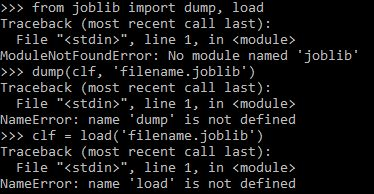
\includegraphics[width=0.75\textwidth]{figures/huda/18.JPG}}\caption{Hasil Tampilan Error.}\end{figure}
\subsubsection{Tuliskan Kode Eror dan Jenis Erornya}
\begin{itemize}
\item \begin{verbatim}from joblib import dump, load\end{verbatim} (Kode baris pertama)
\subitem \begin{verbatim}
Traceback(most recent call last):
 File "<stdin>", line 1, in<module>
ModuleNotFoundError: No module named 'joblib'
\end{verbatim} (Errornya)
\item \begin{verbatim}dump(clf, 'filename.joblib')\end{verbatim} (Kode baris kedua)
\subitem \begin{verbatim}
Traceback(most recent call last):
 File "<stdin>", line 1, in<module>
NameError: name 'dump' is not defined
\end{verbatim} (Errornya)
\item \begin{verbatim}clf = load('filename.joblib')\end{verbatim} (Kode baris ketiga)
\subitem \begin{verbatim}
Traceback(most recent call last):
 File "<stdin>", line 1, in<module>
NameError: name 'load' is not defined
\end{verbatim} (Errornya)
\end{itemize}
\subsubsection{Solusi Pemecahan Masalah Error}
\begin{enumerate}
\item Pada masalah error sebelumnya itu dikarenakan kita belum mempunyai packaged joblib. Jadi solusinya yaitu dengan cara menginstall terlebih dahulu packaged joblibnya setelah itu baru perintah tersebut dapat dijalankan seperti pada gambar 1.2 dan 1.3
\begin{figure}[ht]\centerline{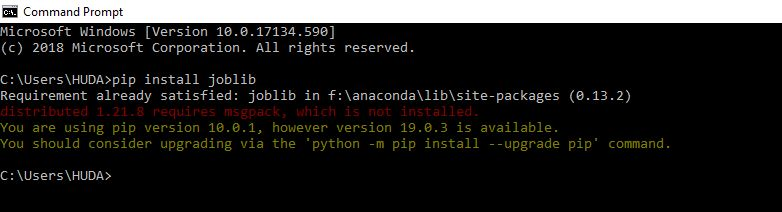
\includegraphics[width=0.75\textwidth]{figures/huda/33.JPG}}\caption{Hasil Tampilan Install joblib.}\end{figure}
\begin{figure}[ht]\centerline{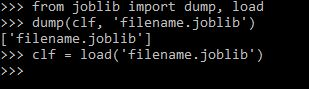
\includegraphics[width=0.75\textwidth]{figures/huda/32.JPG}}\caption{Hasil Tampilan Uji coba perintah joblib.}\end{figure}
\end{enumerate}

\begin{figure}[ht]\centerline{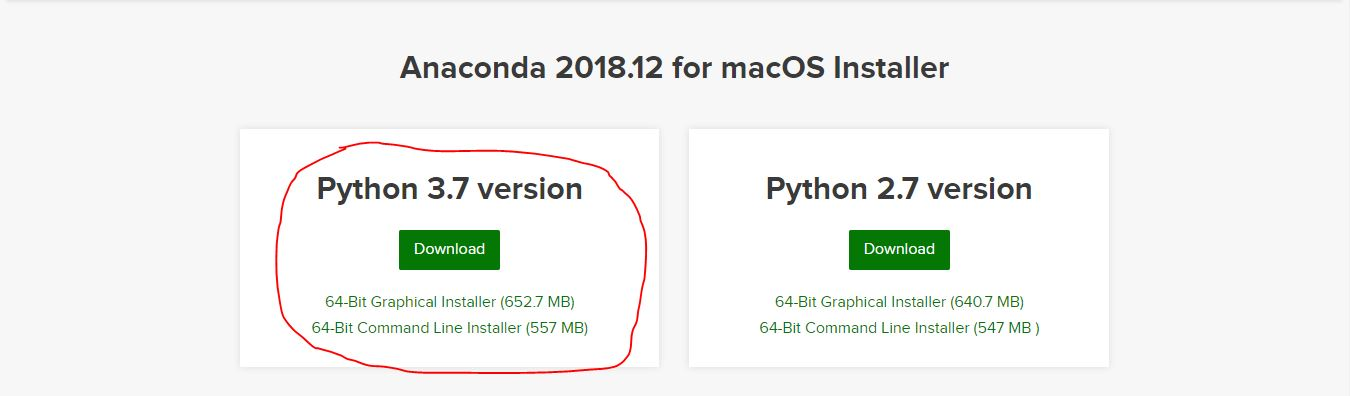
\includegraphics[width=1\textwidth]{figures/huda/1.JPG}}\caption{Download Anaconda.}\end{figure}
\begin{figure}[ht]\centerline{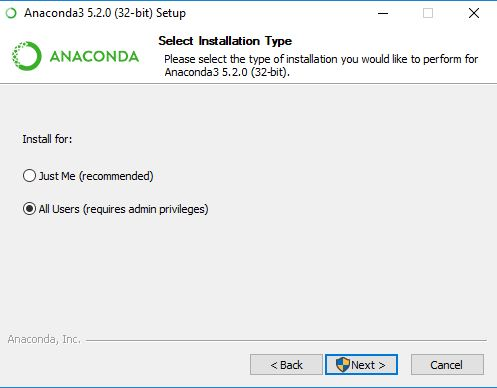
\includegraphics[width=0.75\textwidth]{figures/huda/2.JPG}}\caption{Langkah pertama instalasi anaconda.}\end{figure}
\begin{figure}[ht]\centerline{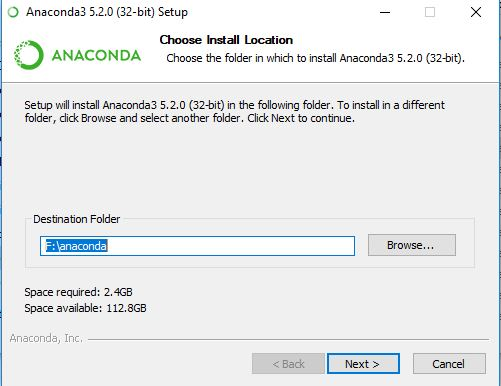
\includegraphics[width=0.75\textwidth]{figures/huda/3.JPG}}\caption{Langkah kedua instalasi anaconda.}\end{figure}
\begin{figure}[ht]\centerline{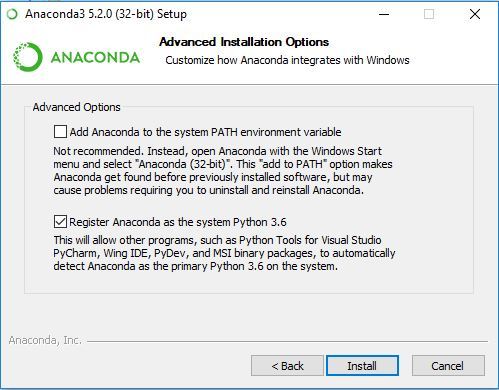
\includegraphics[width=0.75\textwidth]{figures/huda/4.JPG}}\caption{Langkah ketiga instalasi anaconda.}\end{figure}
\begin{figure}[ht]\centerline{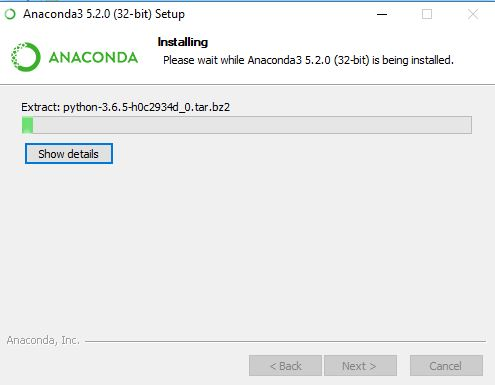
\includegraphics[width=0.75\textwidth]{figures/huda/5.JPG}}\caption{Langkah terakhir instalasi anaconda.}\end{figure}
\begin{figure}[ht]\centerline{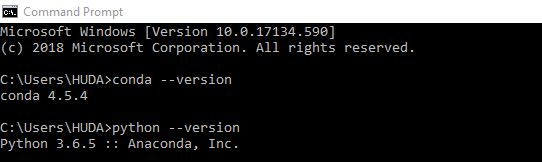
\includegraphics[width=0.75\textwidth]{figures/huda/6.JPG}}\caption{Langkah pertama instalasi scikit pada CMD.}\end{figure}
\begin{figure}[ht]\centerline{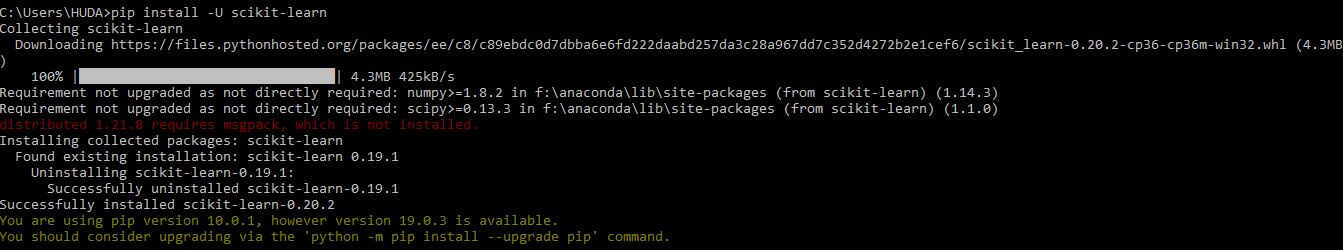
\includegraphics[width=0.75\textwidth]{figures/huda/7.JPG}}\caption{Langkah kedua instalasi scikit pada CMD.}\end{figure}
\begin{figure}[ht]\centerline{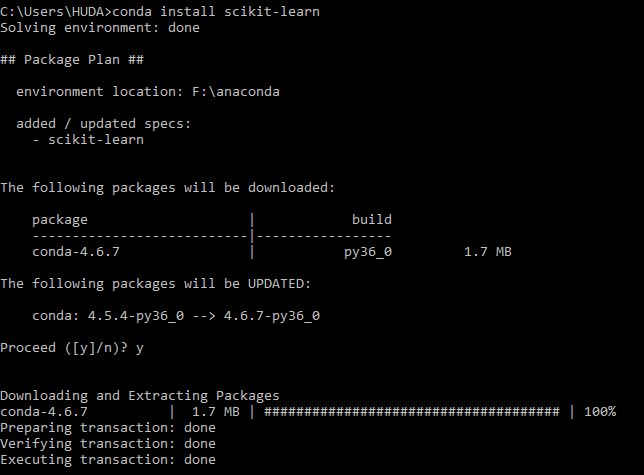
\includegraphics[width=0.75\textwidth]{figures/huda/8.JPG}}\caption{Langkah ketiga instalasi scikit pada CMD.}\end{figure}
\begin{figure}[ht]\centerline{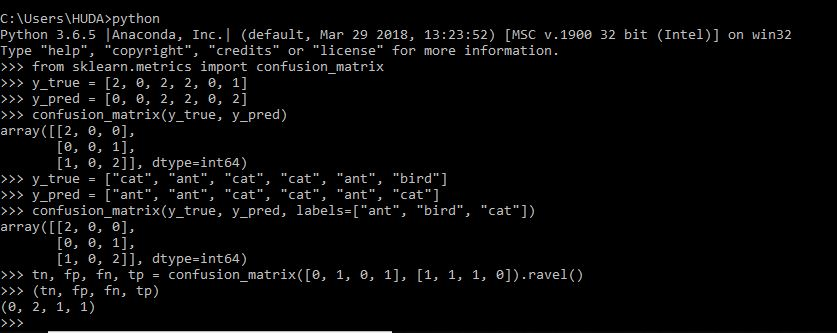
\includegraphics[width=0.75\textwidth]{figures/huda/9.JPG}}\caption{Langkah compile code pada python anaconda.}\end{figure}
\begin{figure}[ht]\centerline{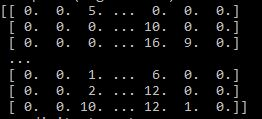
\includegraphics[width=0.75\textwidth]{figures/huda/10.JPG}}\caption{Hasil Tampilan 1.}\end{figure}
\begin{figure}[ht]\centerline{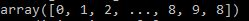
\includegraphics[width=0.75\textwidth]{figures/huda/11.JPG}}\caption{Hasil Tampilan 2.}\end{figure}
\begin{figure}[ht]\centerline{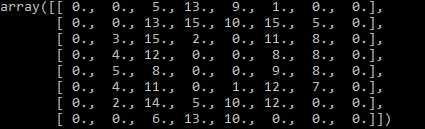
\includegraphics[width=0.75\textwidth]{figures/huda/12.JPG}}\caption{Hasil Tampilan 3.}\end{figure}
\begin{figure}[ht]\centerline{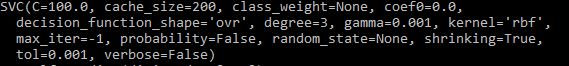
\includegraphics[width=0.75\textwidth]{figures/huda/13.JPG}}\caption{Hasil Tampilan 4.}\end{figure}
\begin{figure}[ht]\centerline{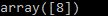
\includegraphics[width=0.75\textwidth]{figures/huda/14.JPG}}\caption{Hasil Tampilan 5.}\end{figure}
\begin{figure}[ht]\centerline{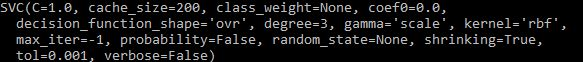
\includegraphics[width=0.75\textwidth]{figures/huda/15.JPG}}\caption{Hasil Tampilan 6.}\end{figure}
\begin{figure}[ht]\centerline{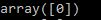
\includegraphics[width=0.75\textwidth]{figures/huda/16.JPG}}\caption{Hasil Tampilan 7.}\end{figure}
\begin{figure}[ht]\centerline{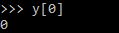
\includegraphics[width=0.75\textwidth]{figures/huda/17.JPG}}\caption{Hasil Tampilan 8.}\end{figure}
\begin{figure}[ht]\centerline{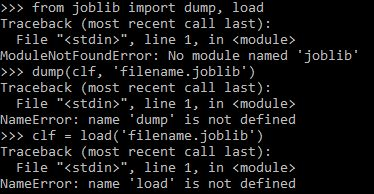
\includegraphics[width=0.75\textwidth]{figures/huda/18.JPG}}\caption{Hasil Tampilan 9.}\end{figure}
\begin{figure}[ht]\centerline{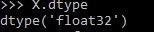
\includegraphics[width=0.75\textwidth]{figures/huda/19.JPG}}\caption{Hasil Tampilan 10.}\end{figure}
\begin{figure}[ht]\centerline{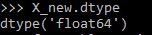
\includegraphics[width=0.75\textwidth]{figures/huda/20.JPG}}\caption{Hasil Tampilan 11.}\end{figure}
\begin{figure}[ht]\centerline{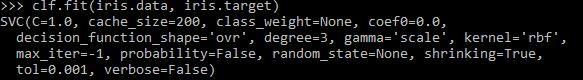
\includegraphics[width=0.75\textwidth]{figures/huda/21.JPG}}\caption{Hasil Tampilan 12.}\end{figure}
\begin{figure}[ht]\centerline{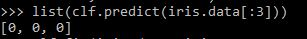
\includegraphics[width=0.75\textwidth]{figures/huda/22.JPG}}\caption{Hasil Tampilan 13.}\end{figure}
\begin{figure}[ht]\centerline{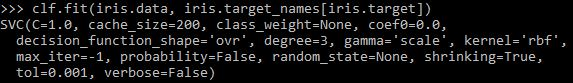
\includegraphics[width=0.75\textwidth]{figures/huda/23.JPG}}\caption{Hasil Tampilan 14.}\end{figure}
\begin{figure}[ht]\centerline{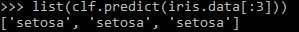
\includegraphics[width=0.75\textwidth]{figures/huda/24.JPG}}\caption{Hasil Tampilan 15.}\end{figure}
\begin{figure}[ht]\centerline{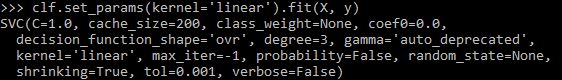
\includegraphics[width=0.75\textwidth]{figures/huda/25.JPG}}\caption{Hasil Tampilan 16.}\end{figure}
\begin{figure}[ht]\centerline{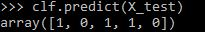
\includegraphics[width=0.75\textwidth]{figures/huda/26.JPG}}\caption{Hasil Tampilan 17.}\end{figure}
\begin{figure}[ht]\centerline{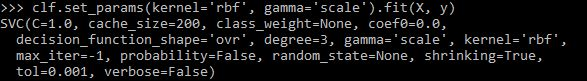
\includegraphics[width=0.75\textwidth]{figures/huda/27.JPG}}\caption{Hasil Tampilan 18.}\end{figure}
\begin{figure}[ht]\centerline{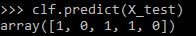
\includegraphics[width=0.75\textwidth]{figures/huda/28.JPG}}\caption{Hasil Tampilan 19.}\end{figure}
\begin{figure}[ht]\centerline{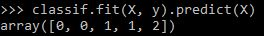
\includegraphics[width=0.75\textwidth]{figures/huda/29.JPG}}\caption{Hasil Tampilan 20.}\end{figure}
\begin{figure}[ht]\centerline{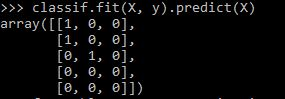
\includegraphics[width=0.75\textwidth]{figures/huda/30.JPG}}\caption{Hasil Tampilan 21.}\end{figure}
\begin{figure}[ht]\centerline{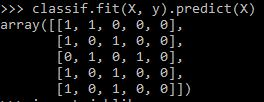
\includegraphics[width=0.75\textwidth]{figures/huda/31.JPG}}\caption{Hasil Tampilan 22.}\end{figure}



\chapter{Related Works}

Your related works, and your purpose and contribution which must be different as below.

\section{Ahmad Syafrizal Huda/1164062}
\subsection{Teori}
\begin{enumerate}
\item Binary Classification yaitu katakanlah kita memiliki tugas untuk mengklasifikasikan objek menjadi dua kelompok berdasarkan beberapa fitur. Sebagai contoh, katakanlah kita diberi beberapa pena dan pensil dari berbagai jenis dan merek, kita dapat dengan mudah memisahkannya menjadi dua kelas, yaitu pena dan pensil.
\subitem Contoh ilustrasi gambar bisa dilihat pada gambar \ref{1}.
\begin{figure}[!htbp]
		\centerline{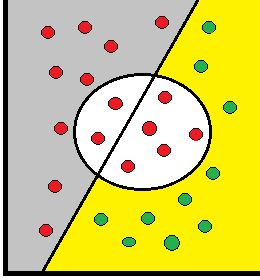
\includegraphics[width=1\textwidth]{figures/huda/binary.JPG}}
		\caption{Binary Classification.}
		\label{1}
\end{figure}
\item Supervised learning merupakan sebuah pendekatan dimana sudah terdapat data yang dilatih, dan terdapat variable yang ditargetkan sehingga tujuan dari pendekatan ini adalah mengkelompokan suatu data ke data yang sudah ada. Sedangkan unsupervised learning tidak memiliki data latih, sehingga dari data yang ada, kita mengelompokan data tersebut menjadi 2 bagian atau 3 bagian dan seterusnya. Dan clustering adalah proses pengelompokan entitas yang sama bersama-sama. Tujuan dari teknik pembelajaran mesin tanpa pengawasan ini adalah untuk menemukan kesamaan pada titik data dan mengelompokkan titik data yang serupa secara bersamaan\cite{zhu2009introduction}.
\subitem Contoh ilustrasi gambar bisa dilihat pada gambar \ref{2}.
\begin{figure}[!htbp]
		\centerline{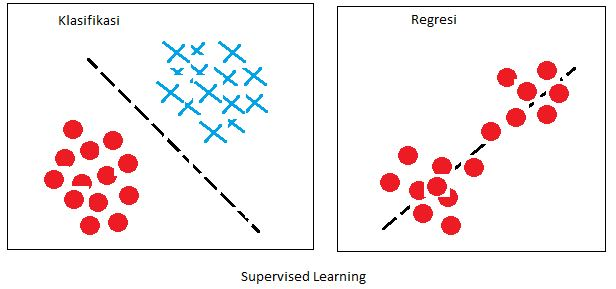
\includegraphics[width=1\textwidth]{figures/huda/supervised.JPG}}
		\caption{Supervised Learning.}
		\label{2}
\end{figure}
\subitem Contoh ilustrasi gambar bisa dilihat  pada gambar \ref{3}.
\begin{figure}[!htbp]
		\centerline{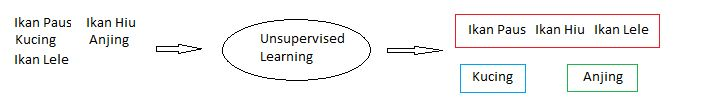
\includegraphics[width=1\textwidth]{figures/huda/unsupervised.JPG}}
		\caption{Unsupervised Learning.}
		\label{3}
\end{figure}
\subitem Contoh ilustrasi gambar bisa dilihat pada gambar \ref{4}.
\begin{figure}[!htbp]
		\centerline{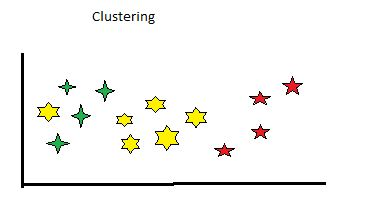
\includegraphics[width=1\textwidth]{figures/huda/clustering.JPG}}
		\caption{Clustering.}
		\label{4}
\end{figure}
\item Evaluasi dan akurasi adalah bagaimana cara kita bisa mengevaluasi sebarapa baik model mengerjakan pekerjaannya dengan cara mengukur akurasinya. Akurasi nantinya didefinisikan sebagai presentase kasus yang telah diklasifikasikan dengan benar. Kita dapat melakukan analisis kesalahan yang telah di buat oleh model.
\subitem Contoh ilustrasi gambar bisa dilihat pada gambar \ref{5}.
\begin{figure}[!htbp]
		\centerline{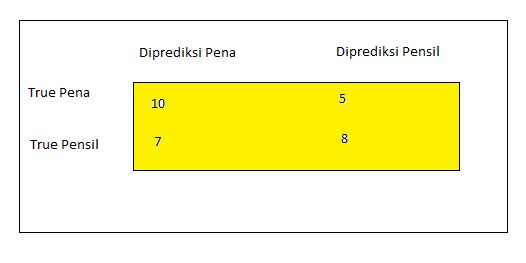
\includegraphics[width=1\textwidth]{figures/huda/evaluasidanakurasi.JPG}}
		\caption{Evaluasi dan Akurasi.}
		\label{5}
\end{figure}
\item Cara membuat dan membaca confusion matrix yaitu, menentukan pokok permasalahan serta atributnya, membuat Decision Tree, membuat Data Testing, mencari nilai variabelnya misal a,b,c, dan d, mencari nilai recall, precision, accuracy, dan erorr rate.
\subitem Contoh Confusion Matrix.
\begin{verbatim}
		Recall =3/(1+3) = 0,75
		Precision = 3/(1+3) = 0,75
		Accuracy =(5+3)/(5+1+1+3) = 0,8
		Error Rate =(1+1)/(5+1+1+3) = 0,2 
\end{verbatim}
\item Berikut ini tata cara kerja K-fold Cross Validation>
	\begin{itemize}
		\item Total instance akan dibagi menjadi N bagian.
		\item Fold yang pertama adalah bagian pertama menjadi testing data dan sisanya menjadi training data.
		\item Hitung akurasi berdasarkan porsi data tersebut dengan menggunakan persamaan.
		\item Fold yang ke dua adalah bagian ke dua menjadi testing data dan sisanya training data. 
		\item Hitung akurasi berdasarkan porsi data tersebut.
		\item Lakukan step secara berulang hingga habis mencapai fold ke-K.
		\item Terakhir hitung rata-rata akurasi K buah.
	\end{itemize}
\subitem Contoh ilustrasi gambar bisa dilihat pada gambar \ref{6}.
\begin{figure}[!htbp]
		\centerline{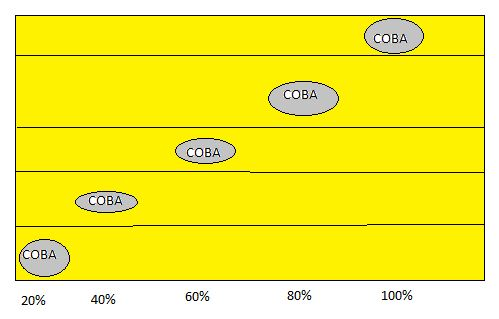
\includegraphics[width=1\textwidth]{figures/huda/K-fold.JPG}}
		\caption{K-fold Cross Validation.}
		\label{6}
\end{figure}
\item Decision Tree adalah sebuah metode pembelajaran yang digunakan untuk melakukan klarifikasi dan regresi. Decision Tree digunakan untuk membuat sebuah model yang dapat memprediksi sebuah nilai variabel target dengan cara mempelajari aturan keputusan dari fitur data. Contoh Decision Tree adalah untuk melakukan predikisi apakah Kuda termasuk hewan mamalia atau bukan.
\subitem Contoh ilustrasi gambar bisa dilihat pada gambar \ref{7}.
\begin{figure}[!htbp]
		\centerline{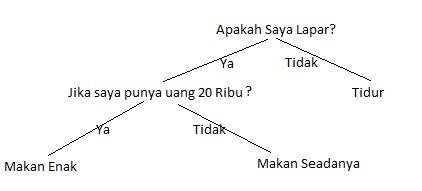
\includegraphics[width=1\textwidth]{figures/huda/DecisionTree.JPG}}
		\caption{Decision Tree.}
		\label{7}
\end{figure}
\item Gain adalah pengurangan yang diharapkan dalam enthropy. Dalam mechine learning, gain dapat digunakan untuk menentukan sebuah urutan atribut atau memperkecil atribut yang telah dipilih. Urutan ini akan membentuk decision tree, atribut gain dipilih yang paling besar. Dan Entropi adalah ukuran ketidakpastian sebuah variabel acak sehingga dapat di artikan entropi adalah ukuran ketidakpastian dari sebuah atribut.
\subitem Contoh ilustrasi gambar bisa dilihat pada gambar \ref{8}.
\begin{figure}[!htbp]
		\centerline{
\includegraphics[width=1\textwidth]{figures/huda/Gain.PNG}}
		\caption{Gain.}
		\label{8}
\end{figure}
\end{enumerate}

\subsection{Scikit-learn}
\begin{enumerate}
\item Penjelasan Codingan ini akan menampilkan data pada file yang ditentukan. Untuk codingan ini file yang dieksekusi untuk digunakan ialah student-mat.csv. Secara jelasnya, dalam codingan dapat dilihat bahwa variabel buahpir didefinisikan untuk pembacaan csv dari " buahnaga  dimana untuk pemisahnya yaitu separation berupa ; . Setelah itu variabel buahpir di tampilkan dengan perintah menampilkan len panjang ataupun jumlah dan hasilnya berupa angka 395 . 
\subitem Gambar Screenshootan codingan dan hasil bisa dilihat pada gambar \ref{9}.
\begin{figure}[!htbp]
		\centerline{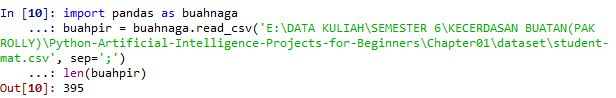
\includegraphics[width=1\textwidth]{figures/huda/1_hari4.JPG}}
		\caption{Hasil Codingan No 1.}
		\label{9}
\end{figure}
\item Penjelasan codingan ini berfungsi untuk menampilkan  baris  G1, G2 dan G3 ( berdasarkan kriterianya ) untuk kolom PASS pada variabel buahpir. Untuk lebih jelasnya, pada codingan terdapat pendefinisian pembacaan lamda ( panjang gelombang ) dari baris G1, G2 dan G3. Apabila row-row tersebut bernilai lebih dari 35 maka akan terdefinisikan angka 1 apabila tidak, maka akan terdefinisikan angka 0 pada kolom PASS ( sesuai permintaan awal ). Selanjutnya variabelnya di ditampilkan sehingga menampilkan keluaran. Tidak lupa terdapat juga jumlah dari baris dan kolom yang terubah sesuai dengan baris yang dieksekusi.
\subitem Gambar Screenshootan codingan dan hasil bisa dilihat pada gambar \ref{10}.
\begin{figure}[!htbp]
		\centerline{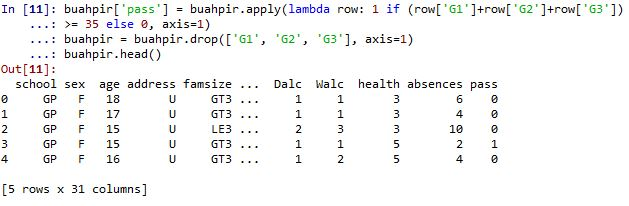
\includegraphics[width=1\textwidth]{figures/huda/2_hari4.JPG}}
		\caption{Hasil Codingan No 2.}
		\label{10}
\end{figure}
\item Penjelasan codingan ini mendefinisikan pemanggilan get dummies dari buahnaga dalam variabel buahpir. Di dalam get dummies sendiri akan terdefinisikan variabel buahpir dengan kolom-kolom yang akan dieksekusi seperti school, address dll. Kemudian variabel tersebut diartikan untuk mendapatkan kembalian berupa keluaran dari eksekusi perintah variabel buahpir beserta dengan jumlah baris dan kolom data yang dieksekusi.
\subitem Gambar Screenshootan codingan dan hasil bisa dilihat pada gambar \ref{11}.
\begin{figure}[!htbp]
		\centerline{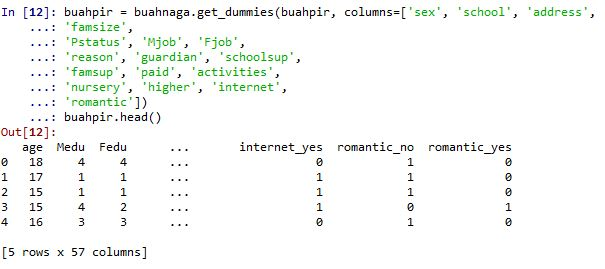
\includegraphics[width=1\textwidth]{figures/huda/3_hari4.JPG}}
		\caption{Hasil Codingan No 3.}
		\label{11}
\end{figure}
\item Penjelasan codingan ini difungsikan untuk mengartikan pembagian data yang berupa training dan testing data. pertama-tama variabel buahpir akan mengartikan sampel yang akan digunakan ( berupa shuffle row ) . Nah kemudian masing-masing parameter yaitu buahpir train dan buahpir test akan berjumlah 500 data ( telah dibagi untuk training dan testing ). Selanjutnya dilakukan pengeksekusian untuk kolom Pass, apabila sesuai dengan axis=1 maka eksekusi fungsi berhasil. Selain itu juga disertakan jumlah dari peserta yang lolos dari semua nilai data setnya.  
\subitem Gambar Screenshootan codingan dan hasil bisa dilihat pada gambar \ref{12}.
\begin{figure}[!htbp]
		\centerline{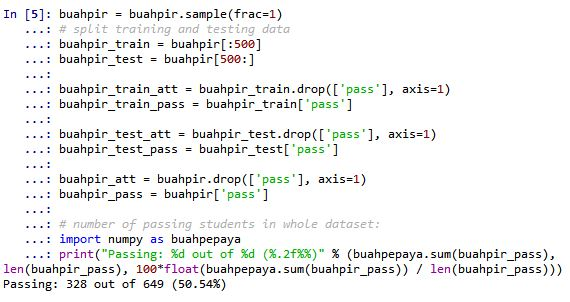
\includegraphics[width=1\textwidth]{figures/huda/4_hari4.JPG}}
		\caption{Hasil Codingan No 4.}
		\label{12}
\end{figure}
\item Penjelasan codingan ini hanya membuktikan pengujian dari Klasifikasi Decision Tree yang ada, apakah true atau tidak dan hasilnya true. Pada codingan ini di definisikan library sklearn untuk mengimpot atau menampilkan tree. Variabel buahapel difungsikan untuk membaca klasifikasi decision tree dari tree itu sendiri dengan 2 parameternya yaitu kriteria=entropy dan max depth=5. Maka selanjutnya variabel buahapel akan masuk dan terbaca dalam module fit dengan 2 parameter yaitu buahpir trai att dan buahpir train pass.
\subitem Gambar Screenshootan codingan dan hasil bisa dilihat pada gambar \ref{13}.
\begin{figure}[!htbp]
		\centerline{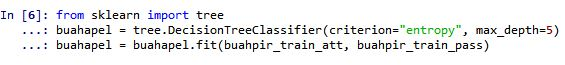
\includegraphics[width=1\textwidth]{figures/huda/5_hari4.JPG}}
		\caption{Hasil Codingan No 5.}
		\label{13}
\end{figure}
\item Penjelasan codingan ini memberikan gambaran dari klasifikasi decision tree yaitu pengolahan parameter yang dieksekusi kedalam variabel buahapel. Tentunya dengan pemanfaatan library graphviz yang telah diimport dan difungsikan.
\subitem Gambar Screenshootan codingan dan hasil bisa dilihat pada gambar \ref{14}.
\begin{figure}[!htbp]
		\centerline{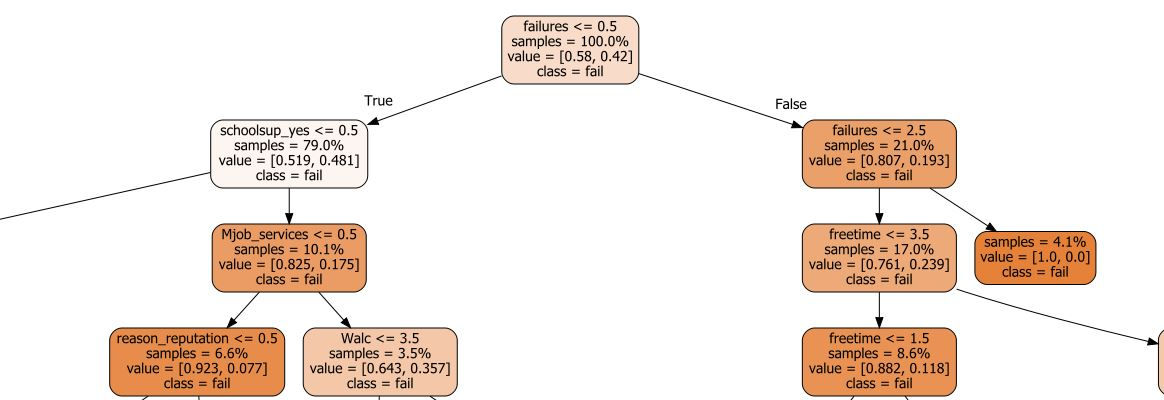
\includegraphics[width=1\textwidth]{figures/huda/6_hari4.JPG}}
		\caption{Hasil Codingan No 6.}
		\label{14}
\end{figure}
\item Penjelasan codingan ini membahas tentang penyimpanan tree dari library graphviz yang dieksekusi bersamaan dengan variabel buahapel dan parameter lainnya. Dilakukan pengecekan dan pengujian apakah klasifikasi decision treenya dapat berjalan atau tidak. Apabila tidak berjalan, maka akan terjadi error, namun codingan ini berfungsi.
\subitem Gambar Screenshootan codingan dan hasil bisa dilihat pada gambar \ref{15}.
\begin{figure}[!htbp]
		\centerline{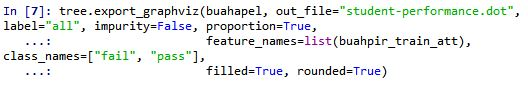
\includegraphics[width=1\textwidth]{figures/huda/7_hari4.JPG}}
		\caption{Hasil Codingan No 7.}
		\label{15}
\end{figure}
\item Penjelasan codingan ini membaca score dari variabel buahapel dimana terdapat 2 parameter yang dihitung dan diuji yaitu buahpir test att dan buahpir test pass. Untuk hasilnya sendiri mengapa berupa angka, dikarenakan pada parameter yang dieksekusi memang memiliki data sehingga dieksekusi dan menghasilkan keluaran dari score tersebut.
\subitem Gambar Screenshootan codingan dan hasil bisa dilihat pada gambar \ref{16}.
\begin{figure}[!htbp]
		\centerline{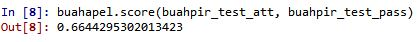
\includegraphics[width=1\textwidth]{figures/huda/8_hari4.JPG}}
		\caption{Hasil Codingan No 8.}
		\label{16}
\end{figure}
\item Penjelasan codingan ini membahas mengenai pengkesekusian fungsi dan variabel dari library yang didefinisikan dan yang diimport. Penjelasan lebih jelasnya ialah codingan ini mendefinisikan library sklearn.model.selection kemudian mengimport cross val score. Kemudian variabel score mendefinisikan cross val score yang telah diimport tadi dengan 4 parameter yaitu buahapel, buahpir att, buahpir pass dan cv=5 untuk dieksekusi. Setelah semua pemrosesan tersebut maka hasil yang di tampilkan ialah rata2 perhitungan dari variabel score dimana dan standar dari plus minusnya tentunya dengan ketentuan parameter Accuracy .
\subitem Gambar Screenshootan codingan dan hasil bisa dilihat pada gambar \ref{17}.
\begin{figure}[!htbp]
		\centerline{\includegraphics[width=1\textwidth]{figures/huda/9_hari4.JPG}}
		\caption{Hasil Codingan No 9.}
		\label{17}
\end{figure}
\item Penjelasan Codingan ini mendefinisikan max depth dalam jarak angka antara parameter 1 dan 20. Variabel buahapel mendefinisikan klasifikasi decision tree dengan 2 parameter. Kemudian variabel score mengeksekusi parameter lainnya yaitu seperti buahapel, buahpir att, buahpir pass dan cv=5 ) . Hasil yang ditampilkan ialah dari max depth, accuracy dan plus minusnya dan akhirnya hasil outputannya keluar.
\subitem Gambar Screenshootan codingan dan hasil bisa dilihat pada gambar \ref{18}.
\begin{figure}[!htbp]
		\centerline{\includegraphics[width=1\textwidth]{figures/huda/10_hari4.JPG}}
		\caption{Hasil Codingan No 10.}
		\label{18}
\end{figure}
\item Penjelasan codingan ini mengartikan bahwa variabel depth\_acc akan mengeksekusi empty dari importan library numphy yang dinamakan buahpepaya dengan 2 parameter yaitu 19,3 dan float. i didefinisikan dengan angka 0 kemudian untuk perhitungan jarak max depth diantara parameter 1 dan 20. Variabel buahapel mengartikan klasifikasi decision tree dengan 2 parameter. setelah itu, variabel score mendefinisikan variabel depth\_acc dengan i dan 0, variabel kedua dari depth\_acc dengan i dan 1 serta variabel ketiga dari depth\_acc dengan i dan 2, maka pengeksekusian akhir bahwa variabel i akan ditambah dengan angka 1 untuk hasil akhirnya. Keluarannya akan berupa array dari perhitungan parameter dan variabel yang telah didefinisikan sebelumnya.
\subitem Gambar Screenshootan codingan dan hasil bisa dilihat pada gambar \ref{19}.
\begin{figure}[!htbp]
		\centerline{\includegraphics[width=1\textwidth]{figures/huda/11_hari4.JPG}}
		\caption{Hasil Codingan No 11.}
		\label{19}
\end{figure}
\item Penjelasan codingan ini mendefinisikan pemanggilan dari library matplotlib.pyplot sebagai buahanggur sehingga nanti hasilnya akan berbentuk gambar grafik/gelombang. Untuk variabel fig dan ax akan mendefinisikan subplots dari buahanggur. Setelah itu ketentuan dari parameter depth acc = 0, depth acc = 1 dan depth acc 2. Selanjutnya untuk menampilkan gelombang maka panggil variabel buahanggur dengan perintah show.
\subitem Gambar Screenshootan codingan dan hasil bisa dilihat pada gambar \ref{20}.
\begin{figure}[!htbp]
		\centerline{\includegraphics[width=1\textwidth]{figures/huda/12_hari4.JPG}}
		\caption{Hasil Codingan No 12.}
		\label{20}
\end{figure}
\end{enumerate}

\subsection{Penanganan Eror}
\begin{enumerate}
\item ScreeShootan Eror pada codingan No 8 dapat dilihat pada gambar \ref{21}.
\subitem 
\begin{figure}[!htbp]
		\centerline{\includegraphics[width=1\textwidth]{figures/huda/eror6.JPG}}
		\caption{Hasil Gambar Eror No 6.}
		\label{21}
\end{figure}
\item Codingan eror dan jenis erornya : sebenarnya tidak terdapat eror pada codingan ini namun saat pertama kali di run current cell codingan ini akan eror dan tidak keluar outputannya dikarenakan library graphviz sebelumnya tidak ditemukan atau belum di install terlebih dahulu.
\subitem 
\begin{verbatim}
import graphviz
dot_data = tree.export_graphviz(buahapel, out_file=None, label="all", impurity=False, proportion=True,
                                feature_names=list(buahpir_train_att), class_names=["fail", "pass"], 
                                filled=True, rounded=True)
graph = graphviz.Source(dot_data)
graph
\end{verbatim}
\item Solusi pemecahan masalah eror tersebut yaitu dengan cara menginstall terlebih dahulu library graphviznya pada anaconda prompt atau command prompt anda dengan perintah conda install graphviz setelah itu run kembali codingan No 8 maka akan muncul outputan atau tampilan keluarannya.
\subitem Berikut gambar cara menginstall graphviz dapat dilihat pada gambar \ref{22}
\begin{figure}[!htbp]
		\centerline{\includegraphics[width=1\textwidth]{figures/huda/penangananeror6.JPG}}
		\caption{Hasil Gambar Penanganan Eror No 6.}
		\label{22}
\end{figure}
\end{enumerate}
\chapter{Methods}

\section{Ahmad Syafrizal Huda / 1164062}
\subsection{Teori}
\begin{enumerate}
\item Random forest ialah sekumpulan classifier yang terdiri dari banyak pohon keputusan dan mengerjakan klasifikasi berdasarkan keluaran dari hasil klasifikasi setiap pohon keputusan anggota. Klasifikasi random forest dikerjakan melalui penggabungan pohon (tree) dengan melakukan training pada sampel data yang dimiliki. Contoh ilustrasi gambar random forest pada gambar \ref{h1}.
\item Cara membaca dataset kasus dan makna setiap file dan isi field masing-masing file
\subitem Gunakan librari pandas yang sudah di install sebelumnya pada python untuk dapat membaca dataset dengan format text file.
\subitem  Selanjutnya buatlah variabel baru misalkan diberi nama dataset yang berisikan perintah untuk membaca file csv.
\begin{verbatim}
import pandas as data
dataset = data.read_csv("car.txt")
dataset.head()
\end{verbatim}
\subitem Pada perintah diatas yaitu memanggil library pandas untuk membaca dataset, membuat variabel dataset yang berisikan data.read\_csv untuk membaca dataset. Pada contoh ini menggunakan txt tapi tetap bisa membaca datasetnya, karena pada saat dijalankan librari pandas secara otomatis akan mengubah data dalam bentuk text file ke format csv. Hasilnya seperti pada gambar \ref{h2}.
\subitem Penjelasan dari isi field pada hasil gambar \ref{h2} yaitu: Atribut Index merupakan atribut otomatis untuk penomoran data yang sudah ada, Atribut Buying merupakan harga beli dari mobil tersebut. dengan value : v high/Sangat mahal,high/mahal,med/Cukup, low/Murah, Atribut Maint merupakan harga perawatan dari mobil tersebut, dengan value sama seperti pada atribut Buying, Atribut Doors merupakan jumlah pintu yang terdapat pada mobil, dengan value 2,3,4,5 more atau lebih dari 5, Atribut Persons merupakan kapasitas orang yang bisa masuk kedapalm mobil, dengan value 2,4, more /lebih, Atribut Lug Boot merupakan ukuran bagasi boot mobil, dengan value small,med,big, Atribut Safety merupakan perkiraan keselamatan mobil, dengan value low,med,high, Yang terakhir yaitu Value, yang dimana merupakan merupakan Class nya atau disebut dengan targetnya menyatakan apakah mobil tersebut dapat diterima atau tidak dan apakah mobil tersebut bagus atau tidak, dengan value unacc, acc, good,v good.
\item Cross validation adalah teknik validasi model untuk menilai bagaimana hasil analisis statistik (model) akan digeneralisasi ke kumpulan data independen. Ini terutama digunakan dalam pengaturan di mana tujuannya adalah prediksi, dan orang ingin memperkirakan seberapa akurat model prediksi akan dilakukan dalam praktek.
\item Arti score 44\% pada random forest yaitu merupakan outputannya untuk hutan acak, arti score 27\% pada decission tree adalah presentasi hasil dari perhitungan dataset acak, dan arti score 29\% dari SVM adalah hasil pendekatan jaringan saraf.  Hasil tersebut didapat dari hasil valdasi silang untuk memastikan bahwa membagi training test dengan cara yang berbeda. Jadi 44\% untuk random forest, 27\% untuk pohon keputusan, dan 29\% untuk SVM. Itu merupakan presentase keakurasian prediksi yang dilakukan pada saat testing menggunakan label pada dataset yang digunakan. Score mendefinisikan aturan evaluasi model.
\item Perhitungan confusion Matriks dapat dilakukan sebagai berikut:
\subitem Import librari Pandas, Matplotlib, dan Numpy.
\subitem Buat variabel x\_aktu yang berisikan data aktual.
\subitem Buat variabel x\_diksi berisikan data yang akan dijadikan sebagai prediksi.
\subitem Buat variabel ak\_confusion yang berisikan crosstab untuk membangun tabel tabulasi silang yang dapat menunjukkan frekuensi kemunculan kelompok data tertentu.
\subitem Pada variabel ak\_confusion definisikan lagi nama baris yaitu Aktual dan kolomnya Prediksi
\subitem Kemudian definisikan suatu fungsi yang diberi nama plot confusion matrix yang berisikan pendefinisian confusion matrix dan juga akan di plotting. untuk code perintah lengkapnya sebagai berikut :
\subitem
\begin{verbatim}
import numpy as cm1
import matplotlib.pyplot as plt
import pandas as cm2
x_aktu = cm2.Series([3, 1, 3, 3, 1, 2, 2, 3, 3, 1, 2, 3], name='Aktual')
x_diksi = cm2.Series([1, 1, 3, 2, 1, 3, 2, 1, 3, 1, 3, 3], name='Prediksi')
ak_confusion = cm2.crosstab(x_aktu, x_diksi)
ak_confusion = cm2.crosstab(x_aktu, x_diksi, rownames=['Aktual'], colnames=['Prediksi'], margins=True)
def plot_confusion_matrix(df_confusion, title='Confusion matrix', cmap=plt.cm.gray_r):
    plt.matshow(ak_confusion, cmap=cmap) # imshow
    #plt.title(title)
    plt.colorbar()
    tick_marks = cm1.arange(len(ak_confusion.columns))
    plt.xticks(tick_marks, ak_confusion.columns, rotation=45)
    plt.yticks(tick_marks, ak_confusion.index)
    #plt.tight_layout()
    plt.ylabel(ak_confusion.index.name)
    plt.xlabel(ak_confusion.columns.name)
plot_confusion_matrix(ak_confusion)
plt.show()
\end{verbatim}
Hasilnya akan seperti pada gambar \ref{h3} :
\item Voting pada random forest sebagaimana voting yaitu suara/hasil untuk setiap target yang diprediksi pada saat melakukan Random Forest. Pertimbangkan target prediksi dengan voting terbanyak/tertinggi sebagai prediksi akhir dari algoritma random forest. Contoh ilustrasi dapat dilihat pada gambar \ref{h4}.
\end{enumerate}

\subsection{Praktek Program}
\begin{enumerate}
\item 
\begin{verbatim}
import pandas as huda
a = huda.Series(['Ahmad', 'Syaf', 'Rizal', 'Huda', 'Mubarrok'],
index = [1, 2, 3, 4, 5])
print (a)
\end{verbatim}
\subitem Baris pertama pada codingan, yaitu import pandas as huda yang artinya kita akan mengimport librari pandas dari python dengan inisiasi huda.
\subitem Baris kedua pada codingan, yaitu Variabel a didefinisikan data data yang sudah dibuat seperti daftar nama dengan menggunakan huda.Series. Series adalah object satu dimensi yang serupa dengan kolom di dalam tabel.
\subitem Baris ketiga pada codingan, yaitu index digunakan untuk melabeli data dengan dimulai dari nomor 1...5, jika tidak label default akan dimulai dari 0,1,2...
\subitem Baris keempat pada codingan, yaitu digunakan untuk mencetak atau menampilkan data pada variabel a yang sudah dibuat sebelumnya.
\subitem Untuk hasilnya dapat dilihat pada gambar \ref{h5}.
\item 
\begin{verbatim}
import numpy as huda
print (huda.arange(50, 101)) 
\end{verbatim}
\subitem Baris pertama pada codingan, yaitu import numpy as huda yang artinya kita akan mengimport librari numpy dari python dengan inisiasi huda.
\subitem Baris kedua pada codingan, yaitu digunakan untuk mencetak atau menampilkan data dengan menggunakan huda.arange untuk membuat array dengan bilangan sekuensial dari mulai nilai awal 50 sampai sebelum 101 dengan berurutan.
\subitem Untuk hasilnya dapat dilihat pada gambar \ref{h6}.
\item 
\begin{verbatim}
import matplotlib.pyplot as huda
huda.plot([0,1,3,5,7,8,10],[25, 35, 30, 45, 50, 45, 30])
huda.show()
\end{verbatim}
\subitem Baris pertama pada codingan, yaitu import matplotlib.pyplot as huda yang artinya kita akan mengimport librari matplotlib dengan class pyplot dari python dengan inisiasi huda.
\subitem Baris kedua pada codingan, yaitu digunakan untuk memasukkan data dengan insiai huda pada class plot dengan nilai x dan y yg sudah ditentukkan.
\subitem Baris ketiga pada codingan, yaitu digunakan untuk mencetak atau menampilkan data dengan inisiai huda.show nantinya keluaranyya berupa grafik.
\subitem Untuk hasilnya dapat dilihat pada gambar \ref{h7}.

\item Menjalankan Klasifikasi Random Forest.
\subitem Pada gambar \ref{h8} berfungsi untuk membaca data yang berupa image\_attribute\_labels dengan format text file. Dengan mendefinisikan variabel imgatt yang berisikan value untuk membaca data, juga menggunakan code untuk skip data yang mengandung bad lines agar tidak terjadi eror pada saat pembacaan file.
\subitem Pada gambar \ref{h9} yaitu mengembalikan baris n teratas (5 secara default) dari dataframe imgatt.
\subitem Pada gambar \ref{h10} yaitu menampilkan beberapa baris dan kolom dari dataframe imgatt.
\subitem Pada gambar \ref{h11} yaitu variabel imgatt2 menggunakan function pivot untuk mengubah kolom jadi baris, dan baris jadi kolom dari dataframe sebelumnya.
\subitem Pada gambar \ref{h12} yaitu imgatt2 head berfungsi untuk mengembalikan nilai teratas dari dataframe imgatt2.
\subitem Pada gambar \ref{h13} yaitu menampilkan beberapa baris dan kolom dari dataframe imgatt2. 
\subitem Pada gambar \ref{h14} yaitu melakukan pivot yang mana imgid menjadi index yang artinya unik.
\subitem Pada gambar \ref{h15} yaitu memuat jawabannya yang berisi apakah burung itu termasuk dalam spesies yang mana. Dua kolomnya terdiri dari imgid dan label.
\subitem Pada gambar \ref{h16} yaitu menunjukkan 11788 baris dan 1 kolom. Dimana kolom itu adalah jenis spesies burungnya.
\subitem Pada gambar \ref{h17} yaitu join antara imgatt2 dengan imglabels dikarenakan isinya sama. Sehingga kita bisa mendapatkan data ciri dan data jawabannya/labelnya sehingga bisa dikategorikan supervised learning.
\subitem Pada gambar \ref{h18} yaitu menghilangkan label yang didepan, dan menggunakan label yang paling belakang yang baru di join.
\subitem Pada gambar \ref{h19} yaitu mengecek 5 data teratas dari df att.
\subitem Pada gambar \ref{h20} yaitu mengecek 5 data teratas dari df label.
\subitem Pada gambar \ref{h21} yaitu 8000 row pertama sebagai data training sisanya sebagai data testing dengan membagi menjadi dua bagian.
\subitem Pada gambar \ref{h22} yaitu memanggil kelas RandomForestClassifier. max features diartikan sebagai berapa banyak kolom pada setiap tree dengan isi maksimum 50.
\subitem Pada gambar \ref{h23} yaitu melakukan fit untuk membangun random forest yang sudah ditentukan dengan maksimum fitur sebanya 50 untuk perpohonnya.
\subitem Pada gambar \ref{h24} yaitu menampilkan hasil prediksi dari random forest sebelumnya.
\subitem Pada gambar \ref{h25} yaitu menampilkan besaran akurasinya dari prediksi diatas atau score perolehan dari klasifikasi.

\item Menjalankan Confusion Matrix.
\subitem Pada gambar \ref{h26} yaitu menyatukan Random Forest ke dalam Confusion Matrix
\subitem Pada gambar \ref{h27} yaitu menampilkan hasil dari gambar sebekumnya dengan array pada perintah cm.
\subitem Pada gambar \ref{h28} yaitu Plotting Confusion Matrix dengan librari Matplotlib.
\subitem Pada gambar \ref{h29} yaitu Set plot sumbunya sesuai dengan nama datanya dan membaca file classes.txt.
\subitem Pada gambar \ref{h30} yaitu Plot hasil perubahan label yang sudah dilakukan.

\item Menjalankan Klasifikasi SVM dan Decision Tree.
\subitem Pada gambar \ref{h31} yaitu klasifikasi dengan decission tree dengan dataset yang sama dan akan muncul akurasi prediksinya.
\subitem Pada gambar \ref{h32} yaitu  klasifikasi dengan SVM dengan dataset yang sama dan akan muncul akurasi prediksinya.
\item Menjalankan Cross Validation.
\subitem Pada gambar \ref{h33} yaitu Cross Validation untuk  Random Forest.
\subitem Pada gambar \ref{h34} yaitu Cross Validation untuk Decission Tree.
\subitem Pada gambar \ref{h35} yaitu Cross Validation untuk SVM.
\item Menjalankan Pengamatan Komponen Informasi.
\subitem Pada gambar \ref{h36} yaitu untuk mengetahui berapa banyak tree yang dibuat, berapa banyak atribut yang dipakai dan informasi lainnya.
\subitem Pada gambar \ref{h37} yaitu hasil dari plotting komponen informasi agar dapat dibaca.
\end{enumerate}

\subsection{Penanganan Eror}
\begin{enumerate}
\item Screenshootan eror ada pada gambar \ref{h38}.
\item 
\begin{verbatim}
from sklearn.model_selection import cross_val_score
scores = cross_val_score(clf, df_train_att, df_train_label, cv=5)
print("Accuracy: %0.2f (+/- %0.2f)" % (scores.mean(), scores.std() * 2))
\end{verbatim}
\subitem 
\begin{verbatim}
scorestree = cross_val_score(clftree, df_train_att, df_train_label, cv=5)
print("Accuracy: %0.2f (+/- %0.2f)" % (scorestree.mean(), scorestree.std() * 2))
\end{verbatim}
\subitem 
\begin{verbatim}
scoressvm = cross_val_score(clfsvm, df_train_att, df_train_label, cv=5)
print("Accuracy: %0.2f (+/- %0.2f)" % (scoressvm.mean(), scoressvm.std() * 2))
\end{verbatim}
\subitem 
\begin{verbatim}
max_features_opts = range(1, 10, 1)
n_estimators_opts = range(2, 40, 4)
rf_params = np.empty((len(max_features_opts)*len(n_estimators_opts),4), float)
i = 0
for max_features in max_features_opts:
    for n_estimators in n_estimators_opts:
        clf = RandomForestClassifier(max_features=max_features, n_estimators=n_estimators)
        scores = cross_val_score(clf, df_train_att, df_train_label, cv=5)
        rf_params[i,0] = max_features
        rf_params[i,1] = n_estimators
        rf_params[i,2] = scores.mean()
        rf_params[i,3] = scores.std() * 2
        i += 1
        print("Max features: %d, num estimators: %d, accuracy: %0.2f (+/- %0.2f)" %
\end{verbatim}
\item Solusi pemecahan masalah tersebut yaitu dengan cara mengubah pada codingan dibawah in yang awalnya datanya 8000 menjadi 1000 semua dan max\_featurenya awalnya 50 menjadi 25.
\subitem 
\begin{verbatim}
df_train_att = df_att[:1000]
df_train_label = df_label[:1000]
df_test_att = df_att[1000:]
df_test_label = df_label[1000:]

df_train_label = df_train_label['label']
df_test_label = df_test_label['label']

from sklearn.ensemble import RandomForestClassifier
clf = RandomForestClassifier(max_features=25, random_state=0, n_estimators=100)
\end{verbatim}
\subitem Jika sudah dilakukan maka langkah selanjutnya yaitu kita tinggal merunning ulang dari awal hingga data tersebut berhasil diajalankan
\end{enumerate}

\begin{figure}
	\centerline{\includegraphics[width=1\textwidth]{figures/huda/chapter3/1.JPG}}
	\caption{Random Forest}
	\label{h1}
\end{figure}

\begin{figure}
	\centerline{\includegraphics[width=1\textwidth]{figures/huda/chapter3/2.PNG}}
	\caption{Hasil Dataset}
	\label{h2}
\end{figure}

\begin{figure}
	\centerline{\includegraphics[width=1\textwidth]{figures/huda/chapter3/3.JPG}}
	\caption{Confusion Matrix}
	\label{h3}
\end{figure}

\begin{figure}
	\centerline{\includegraphics[width=1\textwidth]{figures/huda/chapter3/4.png}}
	\caption{Voting}
	\label{h4}
\end{figure}

\begin{figure}
	\centerline{\includegraphics[width=1\textwidth]{figures/huda/chapter3_praktek/1.JPG}}
	\caption{Aplikasi Menggunakan Pandas}
	\label{h5}
\end{figure}

\begin{figure}[ht]
	\centerline{\includegraphics[width=1\textwidth]{figures/huda/chapter3_praktek/2.JPG}}
	\caption{Aplikasi Menggunakan Numpy}
	\label{h6}
\end{figure}

\begin{figure}[ht]
	\centerline{\includegraphics[width=1\textwidth]{figures/huda/chapter3_praktek/3.JPG}}
	\caption{Aplikasi Menggunakan Matplotlib}
	\label{h7}
\end{figure}

\begin{figure}[ht]
	\centerline{\includegraphics[width=1\textwidth]{figures/huda/chapter3_praktek/4.JPG}}
	\caption{Hasil 1 Random Forest}
	\label{h8}
\end{figure}

\begin{figure}[ht]
	\centerline{\includegraphics[width=1\textwidth]{figures/huda/chapter3_praktek/5.JPG}}
	\caption{Hasil 2 Random Forest}
	\label{h9}
\end{figure}

\begin{figure}[ht]
	\centerline{\includegraphics[width=1\textwidth]{figures/huda/chapter3_praktek/6.JPG}}
	\caption{Hasil 3 Random Forest}
	\label{h10}
\end{figure}

\begin{figure}[ht]
	\centerline{\includegraphics[width=1\textwidth]{figures/huda/chapter3_praktek/7.JPG}}
	\caption{Hasil 4 Random Forest}
	\label{h11}
\end{figure}

\begin{figure}[ht]
	\centerline{\includegraphics[width=1\textwidth]{figures/huda/chapter3_praktek/8.JPG}}
	\caption{Hasil 5 Random Forest}
	\label{h12}
\end{figure}

\begin{figure}[ht]
	\centerline{\includegraphics[width=1\textwidth]{figures/huda/chapter3_praktek/9.JPG}}
	\caption{Hasil 6 Random Forest}
	\label{h13}
\end{figure}

\begin{figure}[ht]
	\centerline{\includegraphics[width=1\textwidth]{figures/huda/chapter3_praktek/10.JPG}}
	\caption{Hasil 7 Random Forest}
	\label{h14}
\end{figure}

\begin{figure}[ht]
	\centerline{\includegraphics[width=1\textwidth]{figures/huda/chapter3_praktek/11.JPG}}
	\caption{Hasil 8 Random Forest}
	\label{h15}
\end{figure}

\begin{figure}[ht]
	\centerline{\includegraphics[width=1\textwidth]{figures/huda/chapter3_praktek/12.JPG}}
	\caption{Hasil 9 Random Forest}
	\label{h16}
\end{figure}

\begin{figure}[ht]
	\centerline{\includegraphics[width=1\textwidth]{figures/huda/chapter3_praktek/13.JPG}}
	\caption{Hasil 10 Random Forest}
	\label{h17}
\end{figure}

\begin{figure}[ht]
	\centerline{\includegraphics[width=1\textwidth]{figures/huda/chapter3_praktek/14.JPG}}
	\caption{Hasil 11 Random Forest}
	\label{h18}
\end{figure}

\begin{figure}[ht]
	\centerline{\includegraphics[width=1\textwidth]{figures/huda/chapter3_praktek/15.JPG}}
	\caption{Hasil 11 Random Forest}
	\label{h19}
\end{figure}

\begin{figure}[ht]
	\centerline{\includegraphics[width=1\textwidth]{figures/huda/chapter3_praktek/16.JPG}}
	\caption{Hasil 12 Random Forest}
	\label{h20}
\end{figure}

\begin{figure}[ht]
	\centerline{\includegraphics[width=1\textwidth]{figures/huda/chapter3_praktek/17.JPG}}
	\caption{Hasil 13 Random Forest}
	\label{h21}
\end{figure}

\begin{figure}[ht]
	\centerline{\includegraphics[width=1\textwidth]{figures/huda/chapter3_praktek/18.JPG}}
	\caption{Hasil 14 Random Forest}
	\label{h22}
\end{figure}

\begin{figure}[ht]
	\centerline{\includegraphics[width=1\textwidth]{figures/huda/chapter3_praktek/19.JPG}}
	\caption{Hasil 15 Random Forest}
	\label{h23}
\end{figure}

\begin{figure}[ht]
	\centerline{\includegraphics[width=1\textwidth]{figures/huda/chapter3_praktek/20.JPG}}
	\caption{Hasil 16 Random Forest}
	\label{h24}
\end{figure}

\begin{figure}[ht]
	\centerline{\includegraphics[width=1\textwidth]{figures/huda/chapter3_praktek/21.JPG}}
	\caption{Hasil 17 Random Forest}
	\label{h25}
\end{figure}

\begin{figure}[ht]
	\centerline{\includegraphics[width=1\textwidth]{figures/huda/chapter3_praktek/22.JPG}}
	\caption{Hasil 1 Confusion Matrix}
	\label{h26}
\end{figure}

\begin{figure}[ht]
	\centerline{\includegraphics[width=1\textwidth]{figures/huda/chapter3_praktek/23.JPG}}
	\caption{Hasil 2 Confusion Matrix}
	\label{h27}
\end{figure}

\begin{figure}[ht]
	\centerline{\includegraphics[width=1\textwidth]{figures/huda/chapter3_praktek/24.JPG}}
	\caption{Hasil 3 Confusion Matrix}
	\label{h28}
\end{figure}

\begin{figure}[ht]
	\centerline{\includegraphics[width=1\textwidth]{figures/huda/chapter3_praktek/25.JPG}}
	\caption{Hasil 4 Confusion Matrix}
	\label{h29}
\end{figure}

\begin{figure}[ht]
	\centerline{\includegraphics[width=1\textwidth]{figures/huda/chapter3_praktek/26.JPG}}
	\caption{Hasil 5 Confusion Matrix}
	\label{h30}
\end{figure}

\begin{figure}[ht]
	\centerline{\includegraphics[width=1\textwidth]{figures/huda/chapter3_praktek/27.JPG}}
	\caption{Hasil 1 Klasifikasi SVM dan Decision Tree}
	\label{h31}
\end{figure}

\begin{figure}[ht]
	\centerline{\includegraphics[width=1\textwidth]{figures/huda/chapter3_praktek/28.JPG}}
	\caption{Hasil 2 Klasifikasi SVM dan Decision Tree}
	\label{h32}
\end{figure}

\begin{figure}[ht]
	\centerline{\includegraphics[width=1\textwidth]{figures/huda/chapter3_praktek/29.JPG}}
	\caption{Hasil 1 Cross Validation}
	\label{h33}
\end{figure}

\begin{figure}[ht]
	\centerline{\includegraphics[width=1\textwidth]{figures/huda/chapter3_praktek/30.JPG}}
	\caption{Hasil 2 Cross Validation}
	\label{h34}
\end{figure}

\begin{figure}[ht]
	\centerline{\includegraphics[width=1\textwidth]{figures/huda/chapter3_praktek/31.JPG}}
	\caption{Hasil 3 Cross Validation}
	\label{h35}
\end{figure}

\begin{figure}[ht]
	\centerline{\includegraphics[width=1\textwidth]{figures/huda/chapter3_praktek/32.JPG}}
	\caption{Hasil 1 Pengamatan Komponen Informasi}
	\label{h36}
\end{figure}

\begin{figure}[ht]
	\centerline{\includegraphics[width=1\textwidth]{figures/huda/chapter3_praktek/33.JPG}}
	\caption{Hasil 2 Pengamatan Komponen Informasi}
	\label{h37}
\end{figure}

\begin{figure}[ht]
	\centerline{\includegraphics[width=1\textwidth]{figures/huda/chapter3_praktek/eror.JPG}}
	\caption{Eror}
	\label{h38}
\end{figure}
\chapter{Experiment and Result}
brief of experiment and result.
\section{Experiment}
Please tell how the experiment conducted from method.

\section{Result}
Please provide the result of experiment

\section{Ahmad Syafrizal Huda/1164062}
\subsection{Teori}
\begin{enumerate}
\item Klasifikasi teks adalah proses pemberian kategori ke dalam teks/dokumen sesuai dengan tipikal dalam supervised machine
\par learning (ML) yang bisa berupa buku perpustakaan, halaman web, artikel media, galeri, dan lain sebagainya. Tujuannya 
\par untuk memberikan label pada setiap teks/dokumen.
\par Contoh ilustrasi gambar dapat dilihat pada gambar \ref{c4_1}
\begin{figure}[ht]
	\centerline{\includegraphics[width=1\textwidth]{figures/huda/chapter4/1.JPG}}
	\caption{Klasifikasi Teks}
	\label{c4_1}
\end{figure}
\item Mengapa klasifikasi bunga tidak dapat menggunakan machine learning? itu dikarenakan memiliki masalah masukan(input) 
\par yang sama tetapi keluarannya (output) yang berbeda, biasanya output yang berbeda ini disebut dengan istilah 'noise'.
\par Noise berarti output yang disimpan bukan seperti seharusnya ( keluaran yang tidak diinginkan ). 
\par Contoh ilustrasi gambar dapat dilihat pada gambar \ref{c4_2}
\begin{figure}[ht]
	\centerline{\includegraphics[width=1\textwidth]{figures/huda/chapter4/2.JPG}}
	\caption{Klasifikasi Bunga}
	\label{c4_2}
\end{figure}
\item Teknik pembelajaran mesin pada teks biasanya menggunakan teknik bag-of-words pada klasifikasi berbasis text dan kata 
\par untuk mengklasifikasikan komentar yang ada diinternet sebagai spam atau bukan. Misalkan pada kolom komentar di youtube
\par dapat di cek seberapa sering suatu kata muncul dalam kalimat. Setiap kata dapat dijadikan baris dan kolomn yang 
\par merupakan kategori kata tersebut, apakah masuk kedalam spam atau tidak. dan contoh lainnya yaitu pada Caption. dimana
\par akan muncul subtitle secara otomatis dari youtube menggunakan sensor suara yang disesuaikan dengan kata yang telah 
\par ditentukan. 
\par Contoh ilustrasi gambar dapat dilihat pada gambar \ref{c4_3}
\begin{figure}[ht]
	\centerline{\includegraphics[width=1\textwidth]{figures/huda/chapter4/3.JPG}}
	\caption{Comment Youtube}
	\label{c4_3}
\end{figure}
\item Vektorisasi data merupakan pembagian dan pemecahan data yang kemudian nantinya data tersebut akan menjadi beberapa data
\par Contoh misalkan dari sebuah paragraph nantinya kan di pecah menjadi beberapa kalimat dari kalimat tersebut dibagi lagi
\par menjadi beberapa kata.
\item Bag-of-words adalah cara untuk merepresentasikan data teks saat memodelkan teks yang menggambarkan kemunculan 
\par kata-kata dalam dokumen dengan algoritma pembelajaran mesin.
\par Contoh ilustrasi gambar dapat dilihat pada gambar \ref{c4_4}
\begin{figure}[ht]
	\centerline{\includegraphics[width=1\textwidth]{figures/huda/chapter4/4.JPG}}
	\caption{Bag Of Words}
	\label{c4_4}
\end{figure}
\item TF-IDF  memberi kita frekuensi kata dalam setiap dokumen atau mengganti data jadi number. Ini adalah rasio berapa 
\par kali kata itu muncul dalam dokumen dibandingkan dengan jumlah total kata dalam dokumen itu. Itu meningkat seiring 
\par jumlah kemunculan kata itu di dalam dokumen meningkat. Setiap dokumen memiliki tf sendiri.
\par Contoh ilustrasi gambar dapat dilihat pada gambar \ref{c4_5}
\begin{figure}[ht]
	\centerline{\includegraphics[width=1\textwidth]{figures/huda/chapter4/5.JPG}}
	\caption{TF-IDF}
	\label{c4_5}
\end{figure}
\end{enumerate}

\subsection{Praktek Program}
\begin{enumerate}
\item Kali ini kita akan membuat data dummy dengan format csv di sini saya mengambil data dari web UCI Machine Learning 
\par Repository dengan nama file Holiday.csv seperti pada gambar \ref{c4_6}
\begin{figure}[ht]
	\centerline{\includegraphics[width=1\textwidth]{figures/huda/chapter4/6.JPG}}
	\caption{Data Dummy 500 Data}
	\label{c4_6}
\end{figure}
\subitem Pada codingan \ref{c4_6} yaitu mengimport librari pandas dimana kita mengaliaskan praktek sebagai pandas. Pandas berguna untuk mengelola  dataframe = matrix = tabel kemudian memanggil nama alias untuk membaca format csvnya.
\item Dari dataframe yang sudah ada sebelumnya kita akan membagi menjadi 2 yaitu 450 row pertama dan 50 row sisanya dapat
\par dilihat pada gambar \ref{c4_7}
\begin{figure}[ht]
	\centerline{\includegraphics[width=1\textwidth]{figures/huda/chapter4/7.JPG}}
	\caption{Membagi 2 Dataframe}
	\label{c4_7}
\end{figure}
\subitem Pada codingan \ref{c4_7} yaitu baris pertama dimana d\_train untuk membagi data training sebanyak 450 row dan pada 
\par baris kedua dimana d\_test untuk data sisa atau data yang baru sebanyak 50 row.
\item Melakukan Vektorisasi dan Klasifikasi Data pada data Eminem pada gambar \ref{c4_8} huda merupakan dataframe keseluruhan dari file csv yang sudah dimasukkan dengan jumlah 448 baris dan 5 kolom. nospam merupakan dataframe yang isinya hanya data yang bukan termasuk spam dengan inisial angka 0. Sedangkan spam merupakan dataframe yang isinya hanya data spam dengan inisial angka 1.
\begin{figure}[ht]
	\centerline{\includegraphics[width=1\textwidth]{figures/huda/chapter4/8.JPG}}
	\caption{Vektorisasi dan Klasifikasi Data}
	\label{c4_8}
\end{figure}
\subitem  Pada gambar \ref{c4_9} merupakan hasil output content dimana terdapat 448 baris/data yang mempunyai 1602 kata-kata \par yang digunakan pada komentar yang ada di content tersebut.
\begin{figure}[ht]
	\centerline{\includegraphics[width=1\textwidth]{figures/huda/chapter4/9.JPG}}
	\caption{Data Content}
	\label{c4_9}
\end{figure}
\subitem Pada gambar \ref{c4_10} maksud dari outputannya merupakan dataframe kata-kata tadi yang berjumlah 1602 kata orang \par yang komen pada data eminem.
\begin{figure}[ht]
	\centerline{\includegraphics[width=1\textwidth]{figures/huda/chapter4/10.JPG}}
	\caption{DataFrame Kata-kata Pada Content}
	\label{c4_10}
\end{figure}
\item Mengklasifikasikan dari data vektorisasi dengan menggunakan klasifikasi svm(support vektorisasi machine) dapat dilihat pada \par gambar \ref{c4_11}.
\begin{figure}[ht]
	\centerline{\includegraphics[width=1\textwidth]{figures/huda/chapter4/11.JPG}}
	\caption{Klasifikasi SVM Dari Data Vektorisasi}
	\label{c4_11}
\end{figure}
\subitem Jadi pada gambar \ref{c4_11} merupakan hasil dari memprediksi data score vektorisasi dengan svm menggunakan metode \par fit dimana digunakan untuk data training atau data pelatihannya saja.
\item Mengklasifikasikan dari data vektorisasi dengan menggunakan klasifikasi Decision Tree dapat dilihat pada gambar \ref{c4_12}.
\begin{figure}[ht]
	\centerline{\includegraphics[width=1\textwidth]{figures/huda/chapter4/12.JPG}}
	\caption{Klasifikasi Decision Tree Dari Data Vektorisasi}
	\label{c4_12}
\end{figure}
\subitem Jadi pada gambar \ref{c4_12} merupakan hasil dari memprediksi data score vektorisasi dengan Decision Tree menggunakan \par metode fit dimana digunakan untuk data training atau data pelatihannya saja.
\item Mengeplot confusion matrix menggunakan matplotlib dapat dilihat pada gambar \ref{c4_13}.
\begin{figure}[ht]
	\centerline{\includegraphics[width=1\textwidth]{figures/huda/chapter4/13.JPG}}
	\caption{Plot Confusion Matrix Menggunakan Matplotlib}
	\label{c4_13}
\end{figure}
\subitem Pada gambar \ref{c4_13} sebelumnya kita harus mengimport matplotlibnya terlebih dahulu setelah itu di sini saya 
\par menggunakan numpy untuk mengeluarkan hasil plot confusion matrix pada matplolibnya nantinya akan keluar normalisasi dari \par confusion matrix berupa data baris dan kolom. 
\item Menjalankan program cross validation pada data vektorisasi dapat dilihat pada gambar \ref{c4_14}.
\begin{figure}[ht]
	\centerline{\includegraphics[width=1\textwidth]{figures/huda/chapter4/14.JPG}}
	\caption{Program Cross Validation Pada Data Vektorisasi}
	\label{c4_14}
\end{figure}
\subitem Pada gambar\ref{c4_14} yang pertama yaitu memunculkan akurasi cross validation dari random forest pada data yang sudah divektorisasi, yang kedua yaitu memunculkan akurasi cross validation dari decision tree pada data yang sudah divektorisasi, dan yang ketiga yaitu memunculkan akurasi cross validation dari svm pada data yang sudah divektorisasi.
\item Membuat program pengamatan komponen informasi pada data yang sudah divektorisasi dapat dilihat pada gambar \ref{c4_15}.
\begin{figure}[ht]
	\centerline{\includegraphics[width=1\textwidth]{figures/huda/chapter4/15.JPG}}
	\caption{Program Pengamatan Komponen Informasi}
	\label{c4_15}
\end{figure}
\subitem Pada gambar \ref{c4_15} merupakan hasil outputan yang mana max features di sana terdapat 9 data dari 10 yang sudah kita masukkan ke dalam codingan sebelumnya dan penomoran estimatornya merupakan data per 5 dari angka 40 sedangkan rata-rata akurasinya kita tuliskan datanya mulai dari 0.9 sampai dengan 1. Titik-titik yang didalam tersebut merupakan data vektorisasi dari pengamatan komponen informasinya.
\end{enumerate}

\subsection{Penanganan Eror}
\begin{enumerate}
\item Pada gambar \ref{c4_16} merupakan ScreeShootan dari data yang eror.
\begin{figure}[ht]
	\centerline{\includegraphics[width=1\textwidth]{figures/huda/chapter4/eror.JPG}}
	\caption{Eror Pada Coding SVM}
	\label{c4_16}
\end{figure}
\item 
\begin{verbatim}
 clfsvm = svm.SVC()
F:\anaconda\lib\site-packages\sklearn\svm\base.py:196: FutureWarning: The default value of gamma will change from 'auto' to 'scale' in version 0.22 to account better for unscaled features. Set gamma explicitly to 'auto' or 'scale' to avoid this warning.
  "avoid this warning.", FutureWarning)
\end{verbatim}
\item Solusi pemecah masalah eror tersebut dengan mengganti dan menambahkan codingan tersebut seperti berikut.
\begin{verbatim}
from sklearn import svm
clfsvm = svm.SVR(gamma='auto')
clfsvm.fit(huda_train_att, huda_train_label)
clfsvm.score(huda_test_att, huda_test_label)
\end{verbatim}
\end{enumerate}
\chapter{Conclusion}
brief of conclusion

\section{Ahmad Syafrizal Huda/1164062}
\subsection{Teori}
\begin{enumerate}
\item Jelaskan Kenapa Kata-Kata harus dilakukan vektorisasi lengkapi dengan ilustrasi gambar.
\subitem Kata kata harus dilakukan vektorisasi dikarenakan untuk mengukur nilai kemunculan suatu kata yang sama dari sebuah kalimat sehingga kata-kata tersebut dapat di prediksi berapa kemunculanya. Atau juga di buatkan vektorisasi data yang digunakan untuk memprediksi bobot dari suatu kata misalkan mobil dan motor sama-sama kendaraan maka akan dibuat prediksi apakah kata tersebut akan muncul pada kalimat yang kira-kira memiliki bobot yang sama. 
\par Untuk ilustrasinya dapat dilihat pada gambar \ref{c5_1}
\begin{figure}[ht]
	\centerline{\includegraphics[width=1\textwidth]{figures/huda/chapter5/1.JPG}}
	\caption{Ilustrasi Soal No. 1}
	\label{c5_1}
\end{figure}
\item Jelaskan Mengapa dimensi dari vektor dataset google bisa mencapai 300 lengkapi dengan ilustrasi gambar.
\subitem Dimensi dari vektor dataset google bisa mencapai 300 karena dimensi dari vektor digunakan untuk membandingkan bobot dari setiap kata, misalkan terdapat kata mobil dan motor pada dataset google tersebut setiap kata tersebut di buat dimensi vektor 300 untuk kata mobil dan 300 dimensi vektor juga untuk kata motor kemudian kata tersebut di bandingkan bobot kesamaan katanya maka akan muncul akurasi sekitar 70an persen kesamaan bobot dikarenakan kata mobil dan motor sama sama di gunakan sebagai kendaraan.
\par Untuk ilustrasinya dapat dilihat pada gambar \ref{c5_2}
\begin{figure}[ht]
	\centerline{\includegraphics[width=1\textwidth]{figures/huda/chapter5/2.JPG}}
	\caption{Ilustrasi Soal No. 2}
	\label{c5_2}
\end{figure}
\item Jelaskan Konsep vektorisasi untuk kata . dilengkapi dengan ilustrasi atau gambar.
\subitem Konesp vektorisasi untuk kata yaitu mengetahui kata tengah dari suatu kalimat utama dengan suatu kalimat contoh ( Jangan lupa like dan comment yah makasih ) kata tengah tersebut merupakan (dan) yang memiliki bobot sebagai kata tengah dari suatu kalimat atau bobot sebagai objek dari suatu kalimat. hal ini sangat berkaitan dengan dimensi vektor pada dataset google yang 300 tadi karena untuk mendapatkan nilai atau bobot dari kata tengah tersebut di dapatkan dari proses dimensiasi dari kata tersebut. 
\par Untuk ilustrasinya dapat dilihat pada gambar \ref{c5_3}
\begin{figure}[ht]
	\centerline{\includegraphics[width=1\textwidth]{figures/huda/chapter5/3.JPG}}
	\caption{Ilustrasi Soal No. 3}
	\label{c5_3}
\end{figure}
\item Jelaskan Konsep vektorisasi untuk dokumen. dilengkapi dengan ilustrasi atau gambar.
\subitem Konsep vektorisasi untuk dokumen hampir sama seperti vektorisasi untuk kata hanya saja pemilihan kata utama atau kata tengah terdapat pada satu dokumen jadi mesin akan membuat dimensi vektor 300 untuk dokumen dan nanti kata tengahnya akan di sandingkan pada dokumen yang terdapat pada dokumen tersebut.
\par Untuk ilustrasinya dapat dilihat pada gambar \ref{c5_4}
\begin{figure}[ht]
	\centerline{\includegraphics[width=1\textwidth]{figures/huda/chapter5/4.JPG}}
	\caption{Ilustrasi Soal No. 4}
	\label{c5_4}
\end{figure}
\item Jelaskan apa mean dan standar deviasi, lengkapi dengan iludtrasi atau gambar.
\subitem Mean adalah nilai rata-rata dari suatu data. Mean disini merupakan petunjuk terhadap kata-kata yang di olah jika kata kata itu akurasinya tinggi berarti kata tersebut sering muncul begitu juga sebaliknya. Standar deviasi merupakan standar untuk menimbang kesalahan. Misalkan kita memperkirakan kedalaman dari dataset merupakan 2 atau 3 tapi pada kenyataanya merupakan 5 itu merupakan kesalahan tapi masih bisa dianggap wajar karena masih mendekati perkiraan awal.
\par Untuk ilustrasinya dapat dilihat pada gambar \ref{c5_5}
\begin{figure}[ht]
	\centerline{\includegraphics[width=1\textwidth]{figures/huda/chapter5/5.JPG}}
	\caption{Ilustrasi Soal No. 5}
	\label{c5_5}
\end{figure}
\item Jelaskan Apa itu Skip-Gram sertakan contoh ilustrasi.
\subitem Skip-Gram yaitu dimana kata tengah menjadi acuan terhadap kata kata pelengkap dalam suatu kalimat.
\par Untuk ilustrasinya dapat dilihat pada gambar \ref{c5_6}
\begin{figure}[ht]
	\centerline{\includegraphics[width=1\textwidth]{figures/huda/chapter5/6.JPG}}
	\caption{Ilustrasi Soal No. 6}
	\label{c5_6}
\end{figure}
\end{enumerate}

\subsection{Praktek Program}
\begin{enumerate}
\item Cobalah dataset google, dan jelaskan vektor dari kata love, faith, fall, sick, clear, shine, bag, car, wash, motor, cycle dan cobalah untuk melakukan perbandingan similirati dari masing-masing kata tersebut. Jelaskan arti dari outputan similaritas.
\subitem Output source code dibawah akan memunculkan data vektor untuk kata love. bahwa vektor memiliki array sebanyak 300 dimensi. Hasil pada source code tersebut dapat dilihat pada gambar \ref{c5_7}.
\begin{verbatim}
gmodel['love']
\end{verbatim}
\begin{figure}[ht]
	\centerline{\includegraphics[width=1\textwidth]{figures/huda/chapter5/7.JPG}}
	\caption{Love}
	\label{c5_7}
\end{figure}
\subitem Output source code dibawah akan memunculkan data vektor untuk kata faith. bahwa vektor memiliki array sebanyak 300 dimensi. Hasil pada source code tersebut dapat dilihat pada gambar \ref{c5_8}.
\begin{verbatim}
gmodel['faith']
\end{verbatim}
\begin{figure}[ht]
	\centerline{\includegraphics[width=1\textwidth]{figures/huda/chapter5/8.JPG}}
	\caption{Faith}
	\label{c5_8}
\end{figure}
\subitem Output source code dibawah akan memunculkan data vektor untuk kata fall. bahwa vektor memiliki array sebanyak 300 dimensi. Hasil pada source code tersebut dapat dilihat pada gambar \ref{c5_9}.
\begin{verbatim}
gmodel['fall']
\end{verbatim}
\begin{figure}[ht]
	\centerline{\includegraphics[width=1\textwidth]{figures/huda/chapter5/9.JPG}}
	\caption{Fall}
	\label{c5_9}
\end{figure}
\subitem Output source code dibawah akan memunculkan data vektor untuk kata sick. bahwa vektor memiliki array sebanyak 300 dimensi. Hasil pada source code tersebut dapat dilihat pada gambar \ref{c5_10}.
\begin{verbatim}
gmodel['sick']
\end{verbatim}
\begin{figure}[ht]
	\centerline{\includegraphics[width=1\textwidth]{figures/huda/chapter5/10.JPG}}
	\caption{Sick}
	\label{c5_10}
\end{figure}
\subitem Output source code dibawah akan memunculkan data vektor untuk kata clear. bahwa vektor memiliki array sebanyak 300 dimensi. Hasil pada source code tersebut dapat dilihat pada gambar \ref{c5_11}.
\begin{verbatim}
gmodel['clear']
\end{verbatim}
\begin{figure}[ht]
	\centerline{\includegraphics[width=1\textwidth]{figures/huda/chapter5/11.JPG}}
	\caption{Clear}
	\label{c5_11}
\end{figure}
\subitem Output source code dibawah akan memunculkan data vektor untuk kata shine. bahwa vektor memiliki array sebanyak 300 dimensi. Hasil pada source code tersebut dapat dilihat pada gambar \ref{c5_12}.
\begin{verbatim}
gmodel['shine']
\end{verbatim}
\begin{figure}[ht]
	\centerline{\includegraphics[width=1\textwidth]{figures/huda/chapter5/12.JPG}}
	\caption{Shine}
	\label{c5_12}
\end{figure}
\subitem Output source code dibawah akan memunculkan data vektor untuk kata bag. bahwa vektor memiliki array sebanyak 300 dimensi. Hasil pada source code tersebut dapat dilihat pada gambar \ref{c5_13}.
\begin{verbatim}
gmodel['bag']
\end{verbatim}
\begin{figure}[ht]
	\centerline{\includegraphics[width=1\textwidth]{figures/huda/chapter5/13.JPG}}
	\caption{Bag}
	\label{c5_13}
\end{figure}
\subitem Output source code dibawah akan memunculkan data vektor untuk kata car. bahwa vektor memiliki array sebanyak 300 dimensi. Hasil pada source code tersebut dapat dilihat pada gambar \ref{c5_14}.
\begin{verbatim}
gmodel['car']
\end{verbatim}
\begin{figure}[ht]
	\centerline{\includegraphics[width=1\textwidth]{figures/huda/chapter5/14.JPG}}
	\caption{Car}
	\label{c5_14}
\end{figure}
\subitem Output source code dibawah akan memunculkan data vektor untuk kata wash. bahwa vektor memiliki array sebanyak 300 dimensi. Hasil pada source code tersebut dapat dilihat pada gambar \ref{c5_15}.
\begin{verbatim}
gmodel['wash']
\end{verbatim}
\begin{figure}[ht]
	\centerline{\includegraphics[width=1\textwidth]{figures/huda/chapter5/15.JPG}}
	\caption{Wash}
	\label{c5_15}
\end{figure}
\subitem Output source code dibawah akan memunculkan data vektor untuk kata motor. bahwa vektor memiliki array sebanyak 300 dimensi. Hasil pada source code tersebut dapat dilihat pada gambar \ref{c5_16}.
\begin{verbatim}
gmodel['motor']
\end{verbatim}
\begin{figure}[ht]
	\centerline{\includegraphics[width=1\textwidth]{figures/huda/chapter5/16.JPG}}
	\caption{Motor}
	\label{c5_16}
\end{figure}
\subitem Output source code dibawah akan memunculkan data vektor untuk kata cycle. bahwa vektor memiliki array sebanyak 300 dimensi. Hasil pada source code tersebut dapat dilihat pada gambar \ref{c5_17}.
\begin{verbatim}
gmodel['cycle']
\end{verbatim}
\begin{figure}[ht]
	\centerline{\includegraphics[width=1\textwidth]{figures/huda/chapter5/17.JPG}}
	\caption{Cycle}
	\label{c5_17}
\end{figure}
\subitem Pada source code dibawah menunjukkan hasil score perbandingan kata apakah kata motor dan cycle memiliki ke samaan atau tidak.  Hasil pada source code tersebut dapat dilihat pada gambar \ref{c5_18}.
\begin{verbatim}
gmodel.similarity('motor','cycle')
\end{verbatim}
\begin{figure}[ht]
	\centerline{\includegraphics[width=1\textwidth]{figures/huda/chapter5/18.JPG}}
	\caption{Similariti Pada Kata Motor dan Cycle}
	\label{c5_18}
\end{figure}
\subitem Pada source code dibawah menunjukkan hasil score perbandingan kata apakah kata wash dan motor memiliki ke samaan atau tidak.  Hasil pada source code tersebut dapat dilihat pada gambar \ref{c5_19}.
\begin{verbatim}
gmodel.similarity('wash','motor')
\end{verbatim}
\begin{figure}[ht]
	\centerline{\includegraphics[width=1\textwidth]{figures/huda/chapter5/19.JPG}}
	\caption{Similariti Pada Kata Wash dan Motor}
	\label{c5_19}
\end{figure}
\subitem Untuk Motor dan Cycle hasilnya adalah 17\%
\subitem Untuk Wash dan Motor hasilnya adalah 10\%
\subitem Artinya Motor dan Cyle memang dalam kategori yang sama misalnya dalam kategori kata-kata yang disatukan/berpasangan. Mesin sudah mengetahui bahwa keduanya dapat dikategorikan sebagai sepasang kata.
\item Jelaskan dengan kata dan ilustrasi fungsi dari extract\_words dan PermuteSentences.
\subitem Extract\_Words merupakan function untuk menambahkan, menghilangkan atau menghapuskan, hal hal yang tidak penting atau tidak perlu di dalam teks. Pada gambar \ref{c5_20} berikut ini menggunakan function extract\_words untuk menghapus komen dengan python style , mencari data yang diinginkan, dan memberikan spasi pada teks.
\begin{figure}[ht]
	\centerline{\includegraphics[width=1\textwidth]{figures/huda/chapter5/20.JPG}}
	\caption{Extract\_Words}
	\label{c5_20}
\end{figure}
\subitem PermuteSentences berfungsi untuk melakukan pengacakan data supaya memperoleh data yang teratur. Ini merupakan class yang digunakan untuk melakukan pengocokan secara acak pada data yang ada. Digunakan cara ini agar tidak terjadi kelebihan memori pada saat dijalankan. Hasilnya dapat dilihat pada gambar \ref{c5_21}.
\begin{figure}[ht]
	\centerline{\includegraphics[width=1\textwidth]{figures/huda/chapter5/21.JPG}}
	\caption{Permute Sentences}
	\label{c5_21}
\end{figure}
\end{enumerate}
\chapter{Discussion}
Please tell more about conclusion and how to the next work of this study.

\section{Ahmad Syafrizal Huda/1164062}
\subsection{Teori}
\begin{enumerate}
\item Jelaskan kenapa file suara harus di lakukan MFCC.
\subitem File suara harus dilakukan MFCC(Mel Frequency Cepstral Coeficients) karena MFCC dapat mengubah file suara/frekuensi suara ke dalam bentuk data vektor yang nantinya akan diolah menjadi outputan dimana telah dilakukan ekstraksi oleh MFCC kemudian direalisasikan sebagai data matrix. Contoh ilustrasi dapat dilihat pada gambar \ref{c6_1}.
\begin{figure}[!htbp]
	\centerline{\includegraphics[width=1\textwidth]{figures/huda/chapter6/1.JPG}}
	\caption{Suara ke MFCC}
	\label{c6_1}
\end{figure} 
\item Jelaskan konsep dasar neural network.
\subitem Neural Network merupakan sistem komputasi yang efisien dimana tema utamanya dipinjam dari analogi jaringan saraf biologis. Neural Network biasa disebut dengan jaringan saraf tiruan dimana Neural Network sebenarnya mengadopsi dari kemampuan otak manusia yang mampu memberikan stimulasi/rangsangan, melakukan proses, dan memberikan output. Contoh ilustrasi dapat dilihat pada gambar \ref{c6_2}.
\begin{figure}[!htbp]
	\centerline{\includegraphics[width=1\textwidth]{figures/huda/chapter6/2.JPG}}
	\caption{Neural Network}
	\label{c6_2}
\end{figure} 
\item Jelaskan konsep pembobotan dalam neural network.
\subitem Sebuah Neural Network dikonfigurasi untuk aplikasi tertentu, seperti pengenalan pola atau klasifikasi data, contohnya pada Neural Network melakukan penyesuaian koneksi sinaptik antar neuron dilakukan dengan menyesuaikan nilai bobot yang ada pada tiap konektivitas baik dari input, neuron maupun output disinkronkan dengan penyesuaian koneksi sinaptik antar neuron itu sendiri. Contoh ilustrasi dapat dilihat pada gambar \ref{c6_3}.
\begin{figure}[!htbp]
	\centerline{\includegraphics[width=1\textwidth]{figures/huda/chapter6/3.JPG}}
	\caption{Pembobotan Neural Network}
	\label{c6_3}
\end{figure} 
\item Jelaskan konsep fungsi aktifasi dalam neural network.
\subitem Fungsi aktivasi dalam neural network yaitu setiap neuron mempunyai tingkat aktivasi yang merupakan fungsi dari input yang masuk padanya. Aktivasi yang dikirim suatu neuron ke neuron lain berupa sinyal dan hanya dapat mengirim sekali dalam satu waktu, meskipun sinyal tersebut disebarkan pada beberapa neuron yang lain. Contoh ilustrasi dapat dilihat pada gambar \ref{c6_4}.
\begin{figure}[!htbp]
	\centerline{\includegraphics[width=1\textwidth]{figures/huda/chapter6/4.JPG}}
	\caption{Aktivasi Neural Network}
	\label{c6_4}
\end{figure} 
\item Jelaskan cara membaca hasil plot dari MFCC.
\subitem Cara membaca hasil plot dari MFCC yaitu Nanti akan ada outputan berbentuk grafik setelah melakukan plot dari MFCC. Kemudian terdapat frekuensi/Hz pada suara frekuensi biasanya vertikal atau biasa disimbolkan dengan sumbu y, Lalu terdapat waktu yang mana waktu diartikan dalam simbol sumbu x. Sedangkan pada bagian dalam atau bisa disimbolkan dengan sumbu z merupakan power atau kekuatan dari lagu atau suara atau desibel yang dihasilkan. Untuk warna biru itu merupakan suara rendah, yang merah merupakan tinggi apabila daya frekuensi nya misalkan suara siul berarti dominan warna merah karena siul biasanya pada nada yang tinggi sedangkan jika bass dominan biru karena bass merupakan nada rendah. Contoh ilustrasi dapat dilihat pada gambar \ref{c6_5}.
\begin{figure}[!htbp]
	\centerline{\includegraphics[width=1\textwidth]{figures/huda/chapter6/5.JPG}}
	\caption{Membaca Hasil Plot dari MFCC}
	\label{c6_5}
\end{figure} 
\item Jelaskan apa itu one-hot encoding.
\par One-hot encoding adalah representasi dari variabel kategori sebagai vektor biner. Yaitu nilai kategorika harusl dipetakan ke nilai integer. Kemudian, setiap nilai integer direpresentasikan sebagai vektor biner yang semuanya bernilai nol kecuali indeks integer, yang ditandai dengan 1. Contoh ilustrasi dapat dilihat pada gambar \ref{c6_6}.
\begin{figure}[!htbp]
	\centerline{\includegraphics[width=1\textwidth]{figures/huda/chapter6/6.JPG}}
	\caption{One-Hot Encoding}
	\label{c6_6}
\end{figure} 
\item Jelaskan apa fungsi dari np.unique dan to\_categorical dalam kode program.
\begin{itemize}
\item np.unique untuk mengekstaksi elemen-elemen unik tertentu dalam array.
\item to\_categorical untuk mengubah vektor kelas yang berupa integer menjadi matriks kelas biner.
\end{itemize}
\begin{figure}[!htbp]
	\centerline{\includegraphics[width=1\textwidth]{figures/huda/chapter6/7.JPG}}
	\caption{np.unique}
\end{figure} 
\begin{figure}[!htbp]
	\centerline{\includegraphics[width=1\textwidth]{figures/huda/chapter6/7_1.JPG}}
	\caption{to\_categorical}
\end{figure} 
\item Jelaskan apa fungsi dari Sequential dalam kode program.
\subitem Fungsi dari Sequential dalam kode program yaitu meruapakan sebuah jenis model yang digunakan dalam perhitungan ataupun code program yang direalisasikan. Neural Networks Sequential membangun fitur tingkat tinggi melalui lapisan yang berurutan. Sequential juga merupakan proses dimana membandingkan setiap elemen larik satu per satu secara beruntun, mulai dari elemen pertama, sampai dengan elemen terakhir atau elemen yang dicari sudah ditemukan.  Contoh ilustrasi dapat dilihat pada gambar \ref{c6_8}.
\begin{figure}[!htbp]
	\centerline{\includegraphics[width=1\textwidth]{figures/huda/chapter6/8.JPG}}
	\caption{One-Hot Encoding}
	\label{c6_8}
\end{figure} 
\end{enumerate}

\subsection{Praktek Program}
\begin{enumerate}
\item Jelaskan isi dari data GTZAN Genre Collection dan data dari freesound. Buat kode program untuk meload data tersebut untuk digunakan pada MFCC.
\subitem Isi dari data GTZAN Genre Collection itu isinya berupa data musik yang sudah di folderkan berdasarkan genre lagunya (dikelompokkan) dengan ekstensi .au yang akan kita lakukan proses MFCC. Sedangakan freesound hanya untuk 1 lagu saja dengan ekstensi .wav.
\lstinputlisting[firstline=1, lastline=2]{src/Jazz.py}
\subitem Code pada baris pertama yaitu Filename jazz merupakan variabel yang berisikan direktori dari file yang dituju, pada code ini digunakan file audio dari genre jazz.
\subitem Code pada baris kedua yaitu Membuat variabel X jazz dan sr jazz yang digunakan untuk meload file dari variabel filename jazz menggunakan librari Librosa dengan durasi 10, yang nantinya akan digunakan pada Mfcc.
\item Jelaskan perbaris kode program dengan kata-kata dan dilengkapi ilustrasi gambar fungsi dari display mfcc() .
\lstinputlisting[firstline=42, lastline=42]{src/Genreidentifier.py}
\subitem Pada kode tersebut menjelaskan display\_mfcc untuk menampilkan vektorisasi dari sebuah suara yang akan menampilkan Plot dan Bar dari inputan code dan file suara hiphop.00028.au.
\item Jelaskan perbaris kode program dengan kata-kata dan dilengkapi ilustrasi gambar fungsi dari extract features song(). Jelaskan juga mengapa yang diambil 25.000 baris pertama?
\lstinputlisting[firstline=42, lastline=42]{src/Genreidentifier.py}
\begin{itemize}
\item Pada kode baris pertama berfungsi untuk memuat inputan. 
\item Pada kode baris kedua itu akan memuat data inputan dengan menggunakan librosa.
\item Kemudian pada parameter inputan yaitu y untuk membuat sebuah fitur pada mfcc.
\item Selanjutnya me-return menjadi array dan akan mengambil 25000 data saja dari hasil vektorisasi dalam 1 lagu yang sudah di display\_mfcc.  
\end{itemize}
\item Jelaskan perbaris kode program dengan kata-kata dan dilengkapi ilustrasi gambar fungsi dari generate features and labels().
\item Jelaskan dengan kata dan praktek kenapa penggunaan fungsi generate features and labels() sangat lama ketika meload dataset genre.
\item Jelaskan kenapa harus dilakukan pemisahan data training dan data set sebesar 80 persen?
\item Praktekkan dan jelaskan masing-masing parameter dari fungsi Sequential().
\item Praktekkan dan jelaskan masing-masing parameter dari fungsi compile() dan tunjukkan keluarannya dengan fungsi summary.
\item Praktekkan dan jelaskan masing-masing parameter dari fungsi fit().
\item Praktekkan dan jelaskan masing-masing parameter dari fungsi evaluate().
\item Praktekkan dan jelaskan masing-masing parameter dari fungsi predict(). 
\end{enumerate}

\subsection{Penanganan Eror}
\begin{enumerate}
\item ScreenShoot Error
\item Tuliskan kode eror dan jenis errornya.
\item Solusi pemecahan masalah error tersebut.
\end{enumerate}

\chapter{Discussion}
Please tell more about conclusion and how to the next work of this study.

\section{Ahmad Syafrizal Huda/1164062}
\subsection{Teori}
\begin{enumerate}
\item Jelaskan kenapa file teks harus di lakukan tokenizer.
\subitem Tokenizer adalah untuk membuat vektor dari teks. Dan mengapa harus dilakukan tokenizer pada file teks? itu karena dengan memfungsikan tokenizer, teks dapat divektorkan. Sehingga teks yang telah telah divektorkan tersebut dapat terbaca pada Machine Learning. Proses tokenizer itu hanya memenggal kata-kata yang ada didalam suatu frasa atau kalimat yang terdapat didalam suatu text dataset. Ilustrasi gambar dapat dilihat pada gambar \ref{c7_1}.
\begin{figure}[!htbp]
	\centerline{\includegraphics[width=1\textwidth]{figures/huda/chapter7/1.JPG}}
	\caption{Tokenizer}
	\label{c7_1}
\end{figure}
\item Jelaskan konsep dasar K Fold Cross Validation pada dataset komentar Youtube pada kode listing \ref{lst:7.0}.
\begin{lstlisting}[caption=K Fold Cross Validation,label={lst:7.0}]
kfold = StratifiedKFold(n_splits=5)
splits = kfold.split(d, d['CLASS'])
\end{lstlisting}
\subitem StartifiedKFold berisikan presentasi sampel untuk setiap kelas. Dimana dalam ilustrasi ini sampel dibagi menjadi 5 dalam setiap class nya. Kemudian sampel tadi akan dimasukan kedalam class dari dataset youtube tadi. Contoh dapat dilihat pada gambar \ref{c7_2}.
\begin{figure}[!htbp]
	\centerline{\includegraphics[width=1\textwidth]{figures/huda/chapter7/2.JPG}}
	\caption{StartifiedKFold}
	\label{c7_2}
\end{figure}
\item Jelaskan apa maksudnya kode program for train, test in splits.
\subitem Maksudnya yaitu untuk menguji apakah setiap data pada dataset sudah di split dan tidak terjadi penumpukan. Yang dimana maksudnya di setiap class tidak akan muncul id yang sama. Ilustrasinya misalkan kita memiliki 4 baju dengan model yang berbeda. Kemudian kita bagikan kedua anak, tentunya setiap anak yang menerima baju tidak memiliki baju yang sama modelnya.
\item Jelaskan apa maksudnya kode program \emph{train\_content = d['CONTENT'].iloc[train\_idx]} dan \emph{test\_content = d['CONTENT'].iloc[test\_idx]}.
\subitem Maksudnya yaitu mengambil data pada kolom atau index CONTENT yang merupakan bagian dari train\_idx dan test\_idx. Ilustrasinya, ketika data telah diubah menjadi train dan test maka kita dapat memilihnya untuk ditampilkan pada kolom yang diinginkan.
\item Jelaskan apa maksud dari fungsi \emph{tokenizer = Tokenizer(num\_words=2000)} dan \emph{tokenizer.fit\_on\_texts(train\_content)}.
\subitem Dimana variabel tokenizer akan melakukan vektorisasi kata menggunakan fungsi Tokenizer yang dimana jumlah kata yang ingin diubah kedalam bentuk token adalah 2000 kata. Dan untuk \emph{tokenizer.fit\_on\_texts(train\_content)} maksudnya kita akan melakukan fit tokenizer hanya untuk dat trainnya saja tidak dengan data test nya untuk kolom CONTENT. Ilustrasinya, Jadi, jika Anda memberikannya sesuatu seperti, "Kucing itu duduk di atas tikar." Ini akan membuat kamus s.t. word\_index ["the"] = 0; word\_index ["cat"] = 1 itu adalah kata -> kamus indeks sehingga setiap kata mendapat nilai integer yang unik.
\item Jelaskan apa maksud dari fungsi \emph{d\_train\_inputs = tokenizer.texts\_to\_matrix(train\_content, mode='tfidf')} dan \emph{d\_test\_inputs = tokenizer.texts\_to\_matrix(test\_content, mode='tfidf')}.
\subitem Maksudnya yaitu untuk variabel d\_train\_inputs akan melakukan tokenizer dari bentuk teks ke matrix dari data train\_content dengan mode matriksnya yaitu tfidf begitu juga dengan variabel d\_test\_inputs untuk data test. Contoh dapat dilihat pada gambar \ref{c7_3}.
\begin{figure}[!htbp]
	\centerline{\includegraphics[width=1\textwidth]{figures/huda/chapter7/3.JPG}}
	\caption{Fungsi Tokenizer}
	\label{c7_3}
\end{figure}
\item Jelaskan apa maksud dari fungsi \emph{d\_train\_inputs = d\_train\_inputs/np.amax(np.absolute(d\_train\_inputs))} dan \emph{d\_test\_inputs = d\_test\_inputs/np.amax(np.absolute(d\_test\_inputs))}.
\subitem Fungsi tersebut akan membagi matrix tfidf tadi dengan amax yaitu mengembalikan maksimum array atau maksimum sepanjang sumbu. Yang hasilnya akan dimasukan kedalam variabel d\_train\_inputs untuk data train dan d\_test\_inputs untuk data test dengan nominal absolut atau tanpa ada bilangan negatif dan koma. Contoh dapat dilihat pada gambar\ref{c7_4}.
\begin{figure}[!htbp]
	\centerline{\includegraphics[width=1\textwidth]{figures/huda/chapter7/4.JPG}}
	\caption{Matrix TFID}
	\label{c7_4}
\end{figure}
\item Jelaskan apa maksud fungsi dari d train outputs = np utils.to categorical(d['CLASS'].iloc[train dan d test outputs = np utils.to categorical(d['CLASS'].iloc[test idx]) dalam kode program.
\subitem maksud dari fungsi tersebut yaitu untuk merubah nilai vektor yang ada pada atribut class menjadi bentuk matrix dengan pengurutan berdasarkan data index training dan testing. Contoh dapat dilihat pada gambar \ref{c7_5}
\begin{figure}[!htbp]
	\centerline{\includegraphics[width=1\textwidth]{figures/huda/chapter7/5.JPG}}
	\caption{Matrix Training dan Testing}
	\label{c7_5}
\end{figure}
\item Jelaskan apa maksud dari fungsi di listing \ref{lst:7.1}. Gambarkan ilustrasi Neural Network nya dari model kode tersebut.
\begin{lstlisting}[caption=Neural Network,label={lst:7.1}]
model=Sequential()
model.add(Dense(512,input_shape=(2000,)))
model.add(Activation('relu'))
model.add(Dropout(0.5))
model.add(Dense(2))
model.add(Act ivation('softmax'))
\end{lstlisting}
\item Jelaskan apa maksud dari fungsi di listing \ref{lst:7.2} dengan parameter tersebut.
\begin{lstlisting}[caption=Model Compile Metric,label={lst:7.2}]
model . compile(loss='categorical_crossentropy',optimizer='adamax',
metrics=[ 'accuracy '])
\end{lstlisting}
\item Jelaskan apa itu Deep Learning.
\subitem Deep Learning merupakan cabang dari Machine Learning atau bagian keluarga yang lebih luas dari method machine learning berdasarkan pada representasi data pembelajaran dan memiliki konsep serupa, tapi dilakukan dengan metode yang lebih cerdas. Deep Learning menggunakan Deep Neural Network dalam menyelesaikan suatu masalah yang terjadi pada Machine Learning.
\item Jelaskan apa itu Deep Neural dan bedanya dengan Deep Learning.
\begin{itemize}
\item Deep Neural Network atau DNN merupakan algoritma yang berbasis neural network yang digunakan untuk mengambil keputusan.
\item Yang membedakan Deep Learning dengan  Deep Neural Network (DNN) adalah DNN merupakan algoritma yang digunakan pada Deep Learning, sedangkan Deep Learning merupakan model yang menggunakan algoritma DNN.
\end{itemize}
\item Jelaskan dengan ilustrasi gambar buatan sendiri(langkah per langkah) bagaimana perhitungan algoritma konvolusi dengan ukuran stride (NPM mod3+1) x (NPM mod3+1) yang terdapat max pooling.
\subitem Konvolusi pada gambar dilakukan dalam image processing untuk menerapkan operator yang memiliki nilai output dari piksel gambar yang berasal dari kombinasi linear nilai input piksel, semakin nilai piksel tersebut maka kualitas gambar bisa semakin bagus. Contoh ilustrasi gambar dapat dilihat pada gambar \ref{c7_6} dan \ref{c7_7}.
\begin{figure}[!htbp]
	\centerline{\includegraphics[width=1\textwidth]{figures/huda/chapter7/6.JPG}}
	\caption{Konvolusi}
	\label{c7_6}
\end{figure}
\begin{figure}[!htbp]
	\centerline{\includegraphics[width=1\textwidth]{figures/huda/chapter7/7.JPG}}
	\caption{Algoritma Perhitungan Konvolusi}
	\label{c7_7}
\end{figure}
\end{enumerate}
\chapter{Discussion}
Please tell more about conclusion and how to the next work of this study.
\chapter{Discussion}
Please tell more about conclusion and how to the next work of this study.
\chapter{Discussion}
Please tell more about conclusion and how to the next work of this study.
\chapter{Discussion}
Please tell more about conclusion and how to the next work of this study.
\chapter{Discussion}
Please tell more about conclusion and how to the next work of this study.
\chapter{Discussion}
Please tell more about conclusion and how to the next work of this study.
\chapter{Discussion}
Please tell more about conclusion and how to the next work of this study.

%now enable appendix numbering format and include any appendices
\appendix
\chapter{Form Penilaian Jurnal}

gambar \ref{form1} dan \ref{form2} merupakan contoh bagaimana reviewer menilai jurnal kita. 
\begin{figure}[ht]
      \centerline{\includegraphics[width=1\textwidth]
      {figures/form1}}
      \caption{Form nilai bagian 1.}
      \label{form1}
      \end{figure}

	\begin{figure}[ht]
	      \centerline{\includegraphics[width=1\textwidth]
	      {figures/form2}}
	      \caption{form nilai bagian 2.}
	      \label{form2}
	      \end{figure}

\chapter{FAQ}

M : Kalo Intership II atau TA harus buat aplikasi ?
D : Ga harus buat aplikasi tapi harus ngoding

M : Pa saya bingung mau ngapain, saya juga bingung mau presentasi apa?
D : Makanya baca de, buka jurnal topik `ganteng' nah kamu baca dulu sehari 5 kali ya, 4 hari udah 20 tuh. Bingung itu tanda kurang wawasan alias kurang baca.

M : Pa saya sudah cari jurnal terindeks scopus tapi ga nemu.
D : Kamu punya mata de? coba dicolok dulu. Kamu udah lakuin apa aja? tolong di list laporkan ke grup Tingkat Akhir. Tinggal buka google scholar klik dari tahun 2014, cek nama jurnalnya di scimagojr.com beres.

M : Pa saya belum dapat tempat intership, jadi ga tau mau presentasi apa?
D : kamu kok ga nyambung, yang dipresentasikan itu yang kamu baca bukan yang akan kamu lakukan.

M : Pa ini jurnal harus yang terindex scopus ga bisa yang lain ?
D : Index scopus menandakan artikel tersebut dalam standar semantik yang mudah dipahami dan dibaca serta bukan artikel asal jadi. Jika diluar scopus biasanya lebih sukar untuk dibaca dan dipahami karena tidak adanya proses review yang baik dan benar terhadap artikel.

M : Pa saya tidak mengerti
D : Coba lihat standar alasan

M : Pa saya bingung
D : Coba lihat standar alasan

M : Pa saya sibuk
D : Mbahmu....

M : Pa saya ganteng
D : Ndasmu....

M : Pa saya kece
D : wes karepmu lah....


Biasanya anda memiliki alasan tertentu jika menghadapi kendala saat proses bimbingan, disini saya akan melakukan standar alasan agar persepsi yang diterima sama dan tidak salah kaprah. Penggunaan kata alasan tersebut antara lain :

1. Tidak Mengerti : anda boleh menggunakan alasan ini jika anda sudah melakukan tahapan membaca dan meresumekan 15 jurnal. Sudah mencoba dan mempraktekkan teorinya dengan mencari di youtube dan google minimal 6 jam sehari selama 3 hari berturut-turut.

2. Bingung : anda boleh mengatakan alasan bingung setelah maksimal dalam berusaha menyelesaikan tugas bimbingan dari dosen(sudah dilakukan semua). Anda belum bisa mengatakan alasan bingung jika anda masih belum menyelesaikan tugas bimbingan dan poin nomor 1 diatas. Setelah anda menyelesaikan tugas bimbingan secara maksimal dan tahap 1 poin diatas, tapi anda masih tetap bingung maka anda boleh memakai alasan ini.

%next line adds the Bibliography to the contents page
\addcontentsline{toc}{chapter}{Bibliography}
%uncomment next line to change bibliography name to references
%\renewcommand{\bibname}{References}
\bibliography{references}        %use a bibtex bibliography file refs.bib
\bibliographystyle{plain}  %use the plain bibliography style

\end{document}

